\chapter{FPGA}
\label{ch:into}

\section{Εισαγωγή}

Τα FPGA (Field Programmable Gate Array) είναι ένας τύπος προγραμματιζόμενου ενσωματομένου κυκλώματος το οποίο μπορεί να προγραμματιστεί πολλές φορές μετά την κατασκευή του.
Τα FPGA ανήκουν σε μία ευρύτερη οικογένεια που ονομάζονται \textbf{προγραμματιζόμενες λογικές συσκευές (Programmable Logic Devices - PLDs)}. 
Αποτελούνται από μία συστοιχία προγραμματιζόμενων λογικών μπλοκ με ένα πλέγμα σύνδεσης, που μπορεί να διαμορφωθεί "επί τόπου" για να διασυνδεθεί με άλλα λογικά μπλοκ 
και να εκτελέσει διάφορες ψηφιακές λειτουργίες. Τα FPGA χρησιμοποιούνται συχνά σε παραγωγή περιορισμένης (χαμηλής) ποσότητας προσαρμοσμένων προϊόντων,
και στην έρευνα και ανάπτυξη, όπου το υψηλότερο κόστος των μεμονωμένων FPGA δεν είναι τόσο σημαντικό, και όπου η δημιουργία και κατασκευή ενός προσαρμοσμένου κυκλώματος
δεν θα ήταν εφικτή υπο τις χρονικές και οικονομικές προυποθέσεις. Άλλες εφαρμογές των FPGA περιλαμβάνουν τους τομείς των τηλεπικοινωνιών, αυτοκινητοβιομηχανίας, αεροδιαστήματος 
και βιομηχανίας, οι οποίοι επωφελούνται από την ευελιξία τους, την υψηλή ταχύτητα επεξεργασίας σήματος και τις ικανότητες παράλληλης επεξεργασίας.

Τα FPGA κατά κανόνα "προγραμματίζονται" - διαμορφώνονται χρησιμοποιώντας \textbf{γλώσσες περιγραφής υλικού (Hardware Description Language - HDL)}, όπως η VHDL και είναι παρόμοιες με αυτές 
που χρησιμοποιούνται για να σχεδιαστούν ολοκληρωμένα κυκλώματα ειδικών εφαρμογών \textbf{(Application-Specific Integrated Circuits - ASICs)}. 
Στις νεότερες γενίες FPGA ξεκίνησε και η υποστήριξη προγραμματισμόυ τους με υψηλότερες γλώσσες περιγραφής κώδικα απο οτι η VHDL ή Verilog οπως είναι η C/C++ 
και αυτον τον τρόπο είναι που εξερευνούμε στην παρούσα διπλωματική εργασία.

Τα λογικά μπλοκ ενός FPGA μπορούν να διαμορφωθούν ώστε να εκτελούν σύνθετες συνδυαστικές λειτουργίες, ή να λειτουργούν ως απλές λογικές πύλες όπως AND και XOR. 
Στα περισσότερα FPGA, τα λογικά μπλοκ περιλαμβάνουν επίσης και στοιχεία μνήμης, τα οποία μπορεί να είναι απο απλά flip-flops εως και πιο εξελιγμένα μπλοκ μνήμης. 
Πολλά FPGA μπορούν να επαναπρογραμματιστούν για να υλοποιήσουν διαφορετικές λειτουργίες, επιτρέποντας ευέλικτη επαναδιαμορφώσιμη όπως και στο λογισμικό υπολογιστών.

Τα FPGA έχουν επίσης ρόλο στην ανάπτυξη ενσωματωμένων συστημάτων λόγω της δυνατότητάς τους να ξεκινούν την ανάπτυξη λογισμικού συστήματος ταυτόχρονα με το υλικό, 
να επιτρέπουν προσομοιώσεις απόδοσης συστήματος σε πολύ πρώιμο στάδιο της ανάπτυξης, και να επιτρέπουν διάφορες δοκιμές συστήματος και επαναλήψεις σχεδιασμού 
πριν την τελική διαμόρφωση της αρχιτεκτονικής του συστήματος.

Τα FPGA χρησιμοποιούνται επίσης συχνά κατά την ανάπτυξη ASICs για την επιτάχυνση της διαδικασίας προσομοίωσης καθώς τα κυκλώματα πρώτα δοκιμάζονται στα fpga και αφού 
οι δοκιμές σε Hardware In The Loop είναι επιτυχείς τότε εκκινείται η διαδικασία κατασκευής του ολοκληρωμένου κυκλώματος ASIC. 

Στην παρακάτω εικόνα φαίνεται ενδεικτικά ένας ολοκληρωμένο FPGA συστημα της Xilinx η οποία αποτελεί πλέον μια απο τις μεγαλύτερες εταιρείες παραγωγής αλλά
και έρευνας/ανάπτυξης τους.

\begin{figure}[h!]
  \centering
  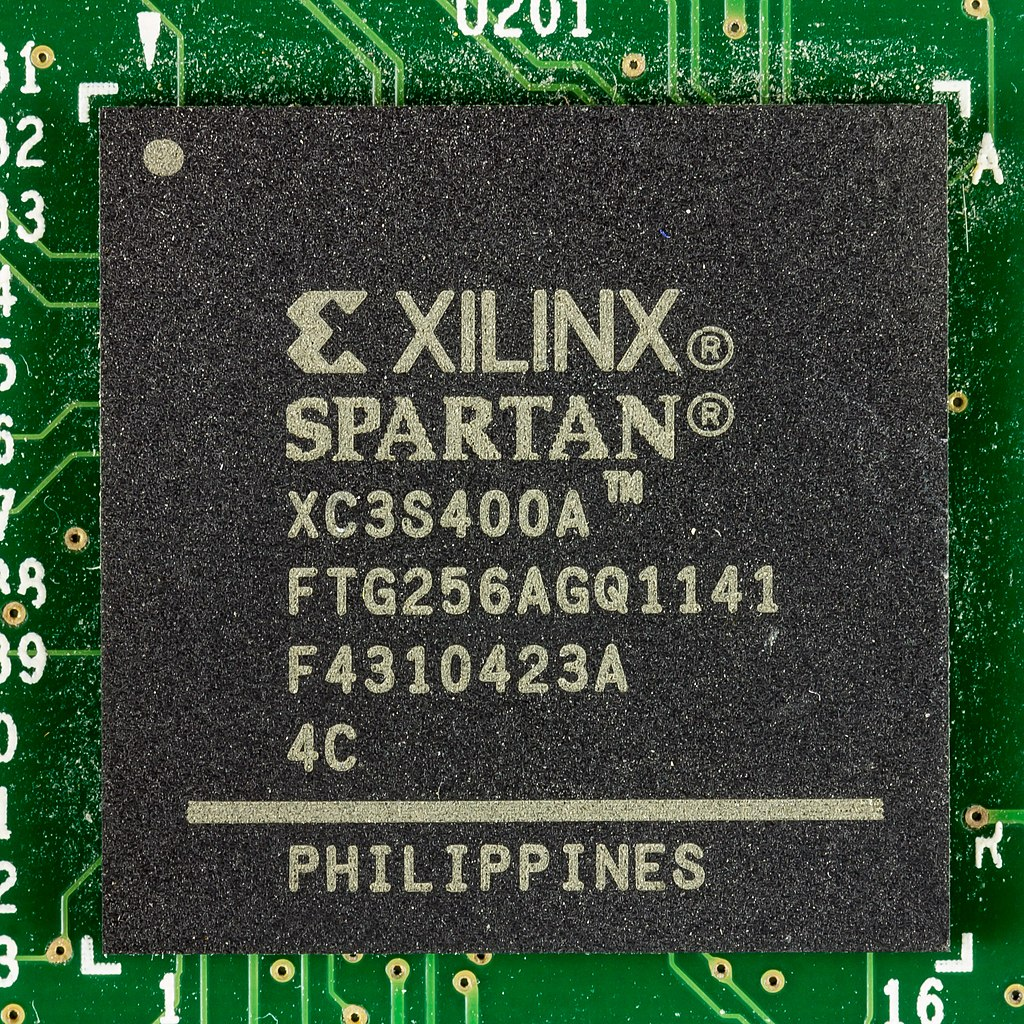
\includegraphics[width=0.8\textwidth]{figures/chapter3/xilinx_fpga.png}
  \caption{Xilinx FPGA IC}
  \label{fig:xilinx_fpga}
\end{figure}

Μέχρι το 2013, η Altera 31\%, η Xilinx 36\% και η Actel 10\% αντιπροσώπευαν μαζί περίπου το 77\% της αγοράς FPGA.
\begin{table}[h!]
  \centering
  \begin{tabular}{|c|c|}
    \hline
    \textbf{Εταιρεία} & \textbf{Ποσοστό Αγοράς (\%)} \\
    \hline
    Altera & 31 \\
    Xilinx & 36 \\
    Actel & 10 \\
    Υπολοιπες & 33 \\
    \hline
    \textbf{Σύνολο} & 100 \\
    \hline
  \end{tabular}
  \caption{Ποσοστά αγοράς FPGA μέχρι το 2013}
  \label{tab:fpga_market_share}
\end{table}

\section{Ιστορική Εξέλιξη των FPGA}
Η βιομηχανία των FPGA ξεκίνησε από τις προγραμματιζόμενες μνήμες μόνο ανάγνωσης (PROM) και τις προγραμματιζόμενες λογικές συσκευές (PLDs). 
Οι PROMs και τα PLDs είχαν την επιλογή να προγραμματίζονται είτε σε παρτίδες στο εργοστάσιο είτε στο πεδίο (field-programmable).

\subsection{Πρωτο FPGA}
Ο πρώτος κατασκευαστής FPGA ήταν η εταιρεία Altera η οποία ιδρύθηκε το 1983 και παρουσίασε την πρώτη επαναπρογραμματιζόμενη λογική συσκευή της βιομηχανίας το 1984,
την γνωστή EP300 η οποία διέθετε ένα μικρό παραθυράκι στη συσκευασία και εδινε την επιλογή στους χρήστες να χρησιμοποιούν την υπεριώδη ακτινοβολία 
για να διαγράφουν τα κύτταρα μνήμης της EPROM που περιείχαν τις ρυθμίσεις της συσκευής.

\begin{figure}[h!]
  \centering
  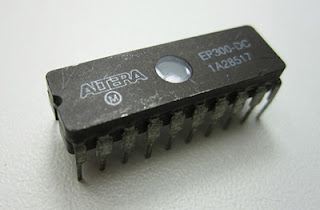
\includegraphics[width=0.8\textwidth]{figures/chapter3/altera_first_fpga.png}
  \caption{Altera first FPGA with erasable EPROM}
  \label{fig:altera_first_fpga}
\end{figure}

Η Xilinx παρήγαγε το πρώτο εμπορικά βιώσιμο FPGA το 1985 αποκαλούμενο XC2064. 
Το XC2064 διέθετε προγραμματιζόμενες πύλες και προγραμματιζόμενες συνδέσεις μεταξύ των πυλών, αποτελώντας την αρχή μιας νέας τεχνολογίας και αγοράς.
Το XC2064 είχε 64 διαμορφώσιμα λογικά μπλοκ (CLBs), με δύο πίνακες αναζήτησης (LUTs) τριών εισόδων.

https://www.righto.com/2020/09/reverse-engineering-first-fpga-chip.html
take data from here also και add some images

\subsection{Εξέλιξη των FPGA μετά το XC2064}
Το 1987, το Naval Surface Warfare Center στην Αμερική χρηματοδότησε ένα πείραμα που πρότεινε ο Steve Casselman για την ανάπτυξη ενός υπολογιστή που
θα υλοποιούσε 600.000 επαναπρογραμματιζόμενες πύλες. Ο Casselman ήταν επιτυχής και ένα δίπλωμα ευρεσιτεχνίας σχετικό με το σύστημα εκδόθηκε το 1992.

Η Altera και η Xilinx συνέχισαν χωρίς ανταγωνισμό και αναπτύχθηκαν γρήγορα από το 1985 έως τα μέσα της δεκαετίας του 1990, όταν εμφανίστηκαν ανταγωνιστές,
μειώνοντας σημαντικά το μερίδιο αγοράς τους. Μέχρι το 1993, η Actel (αργότερα Microsemi, τώρα Microchip) εξυπηρετούσε περίπου το 18\% της αγοράς.

Η δεκαετία του 1990 ήταν μια περίοδος ταχείας ανάπτυξης για τα FPGA, τόσο σε πολυπλοκότητα κυκλωμάτων όσο και σε όγκο παραγωγής.
Στις αρχές της δεκαετίας του 1990, τα FPGA χρησιμοποιούνταν κυρίως στις τηλεπικοινωνίες και τα δίκτυα
και μέχρι το τέλος της δεκαετίας, τα FPGA βρήκαν εφαρμογή σε καταναλωτικά, αυτοκινητοβιομηχανικά και βιομηχανικά προϊόντα.

\subsection{Απο απλά LUT-Based σε μοντέρνες ετερόγενες αρχιτεκτονικές}
Τα αρχικά FPGA βασίζονταν κυρίως σε απλές δομές LUT (Look-Up Tables) και στοιχεία μνήμης.
Η αρχιτεκτονική αυτών των πρώτων συσκευών περιλάμβανε συστοιχίες από λογικά κελιά, όπου κάθε κελί περιείχε ένα LUT (συνήθως 4 εισόδων) και ένα flip-flop.
Τα LUTs ακόμα και τώρα είναι ένα απο τα σημαντικότερα στοιχεία των FPGA, επιτρέποντας στους προγραμματιστές να υλοποιούν ειδικά λογικά κυκλώματα με ευελιξία χωρίς να χρειάζεται να σχεδιάσουν φυσικά κυκλώματα.
Η βασική λειτουργία ενός LUT (Look-Up Table) σε ένα FPGA είναι να αποθηκεύει έναν πίνακα αληθείας που αντιστοιχίζει συνδυασμούς εισόδων σε τιμές εξόδου.
Ο αριθμός των εισόδων και εξόδων για ένα LUT μπορεί να διαφέρει ανάλογα με τη συγκεκριμένη αρχιτεκτονική FPGA.
Τα σύγχρονα FPGAs συνήθως διαθέτουν LUTs με τέσσερις ή έξι εισόδους, αν και ορισμένες αρχιτεκτονικές υποστηρίζουν LUTs με έως και οκτώ εισόδους.


Τα LUTs των FPGA είναι εξαιρετικά ευέλικτα και μπορούν να χρησιμοποιηθούν για ένα ευρύ φάσμα εφαρμογών, συμπεριλαμβανομένης της ψηφιακής επεξεργασίας σήματος, της υπολογιστικής όρασης και της μηχανικής μάθησης. Χρησιμοποιούνται επίσης συχνά σε συστήματα βιομηχανικού αυτοματισμού και ελέγχου, καθώς και σε τηλεπικοινωνιακό και δικτυακό εξοπλισμό.

Τα LUTs στα σύγχρονα FPGA συνδυάζονται συχνά με flip-flops, πολλαπλασιαστές, και άλλα κυκλώματα για να σχηματίσουν το βασικό δομικό στοιχείο που ονομάζεται CLB (Configurable Logic Block) ή LAB (Logic Array Block). Κάθε CLB μπορεί να περιλαμβάνει πολλαπλά LUTs και flip-flops, ανάλογα με την αρχιτεκτονική του FPGA.

Για παράδειγμα, στην οικογένεια Xilinx UltraScale+, κάθε CLB περιλαμβάνει οκτώ 6-input LUTs και δεκαέξι flip-flops. Αυτά τα CLBs είναι διατεταγμένα σε μια συστοιχία και διασυνδέονται μέσω ενός προγραμματιζόμενου δικτύου διασύνδεσης.

\paragraph{Διαμόρφωση και Αποδοτικότητα των LUT}
Τα LUTs στα FPGAs μπορούν να διαμορφωθούν με διάφορους τρόπους για την αύξηση της αποδοτικότητας:

\begin{itemize}
  \item \textbf{Fracturable LUTs}: Ένα μεγάλο LUT (π.χ., 6-input) μπορεί να "διασπαστεί" σε μικρότερα LUTs (π.χ., δύο 5-input LUTs) υπό ορισμένες συνθήκες.
  
  \item \textbf{Distributed RAM}: Τα LUTs μπορούν να χρησιμοποιηθούν ως μικρές μονάδες μνήμης RAM, επιτρέποντας την υλοποίηση μικρών, διεσπαρμένων μνημών με χαμηλή καθυστέρηση.
  
  \item \textbf{Shift Registers}: Τα LUTs μπορούν να διαμορφωθούν ως καταχωρητές ολίσθησης, επιτρέποντας την αποδοτική υλοποίηση λειτουργιών καθυστέρησης και FIFO.
\end{itemize}

Με τη συνεχιζόμενη ανάπτυξη της αγοράς FPGA, τα LUTs είναι πιθανό να παραμείνουν κρίσιμο συστατικό του σχεδιασμού ψηφιακών κυκλωμάτων για πολλά χρόνια ακόμη, προσαρμοζόμενα διαρκώς στις εξελισσόμενες ανάγκες των σύγχρονων εφαρμογών ψηφιακής επεξεργασίας.
Ωστόσο, με την πρόοδο της τεχνολογίας, η αρχιτεκτονική των FPGA εξελίχθηκε δραματικά σε ετερογενείς αρχιτεκτονικές που υποστηρίζουν πολύπλοκες εφαρμογές.

\subsubsection{Η Εξέλιξη των Αρχιτεκτονικών FPGA}

Η εξέλιξη των FPGA ακολούθησε μια σταδιακή πορεία προσθήκης εξειδικευμένων πόρων:

\begin{itemize}
  \item \textbf{Ενσωματωμένη Μνήμη}: Οι κατασκευαστές άρχισαν να προσθέτουν μπλοκ μνήμης (RAM blocks) για την αποθήκευση δεδομένων, αυξάνοντας ταχύτητα πρόσβασης και χωρητικότητα.
  
  \item \textbf{Προσθήκη Πολλαπλασιαστών}: Η εισαγωγή αποκλειστικών πολλαπλασιαστών στη δεκαετία του 2000 επέτρεψε αποδοτικότερους υπολογισμούς DSP.
  
  \item \textbf{DSP Slices}: Τα σύγχρονα FPGA διαθέτουν εξειδικευμένα μπλοκ DSP που συνδυάζουν πολλαπλασιαστές, αθροιστές και καταχωρητές για αποδοτικές μαθηματικές λειτουργίες.
  
  \item \textbf{Hard Processor Cores}: Η ενσωμάτωση επεξεργαστών ARM (όπως στις σειρές Zynq της Xilinx και SoC FPGA της Intel) δημιούργησε υβριδικά συστήματα που συνδυάζουν την ευελιξία του FPGA με τη λειτουργικότητα ενός μικροεπεξεργαστή.
  
  \item \textbf{Transceivers Υψηλής Ταχύτητας}: Προσθήκη πομποδεκτών για επικοινωνίες υψηλής ταχύτητας (έως 112G PAM4 στις νεότερες συσκευές).
  
  \item \textbf{HBM Memory}: Η προσθήκη μνήμης HBM (High-Bandwidth Memory) στο ίδιο πακέτο με το FPGA επιτρέπει εξαιρετικά υψηλό εύρος ζώνης μνήμης.
  
  \item \textbf{Επιταχυντές ΑΙ}: Εξειδικευμένοι πυρήνες για επιτάχυνση εφαρμογών τεχνητής νοημοσύνης και βαθιάς μάθησης.
\end{itemize}

Περισσότερες λεπτομέρειες σχετικά με τα δομικά στοιχεία των FPGA, θα δοθούν σε μεταγενέστερη ενότητα \textbf{Δομικά Στοιχεία FPGA}~\ref{sec:fpga_building_blocks}.

\subsection{Σύγχρονες Ετερογενείς Αρχιτεκτονικές}

\textbf{Xilinx UltraScale+ Architecture}

Η αρχιτεκτονική UltraScale+ της Xilinx (τώρα AMD) αποτελεί ένα εξαιρετικό παράδειγμα σύγχρονης ετερογενούς αρχιτεκτονικής FPGA. Συγκεκριμένα περιλαμβάνει:

\begin{itemize}
  \item Τεχνολογία κατασκευής 16nm FinFET για μειωμένη κατανάλωση και αυξημένη απόδοση
  \item Βελτιστοποιημένα CLB (Configurable Logic Blocks) με 6-input LUTs
  \item Ενσωματωμένα DSP slices (DSP48E2) ικανά για πράξεις 27×18-bit πολλαπλασιασμού-συσσώρευσης
  \item UltraRAM: συμπαγή μπλοκ μνήμης 288 Kb για αποδοτικότερη υλοποίηση μεγάλων μνημών
  \item Transceivers έως 32.75 Gbps
  \item Επιλογές για ενσωματωμένους επεξεργαστές ARM Cortex-A53 και Cortex-R5 (στα Zynq UltraScale+)
  \item Πυρήνες HBM2 για εφαρμογές υψηλού εύρους ζώνης μνήμης
\end{itemize}

\textbf{Intel Stratix 10 Architecture}

Η αρχιτεκτονική Stratix 10 της Intel αποτελεί την αντίστοιχη προηγμένη πλατφόρμα:

\begin{itemize}
  \item Τεχνολογία 14nm TriGate FinFET της Intel
  \item Τεχνολογία HyperFlex με καταχωρητές Hyper-Registers για βελτιστοποίηση χρονισμού και απόδοσης
  \item Ενσωματωμένους τετραπύρηνους επεξεργαστές ARM Cortex-A53
  \item DSP μπλοκ που υποστηρίζουν πράξεις με υψηλή παραλληλία
  \item Transceivers έως 58G PAM4
  \item Διεπαφές μνήμης DDR4 έως 2666 Mbps
  \item Τεχνολογία Embedded Multi-Die Interconnect Bridge (EMIB) για προσαρμοσμένες διαμορφώσεις
  \item Υποστήριξη για στοίβες μνήμης HBM2
\end{itemize}

\subsection{Επόμενη Γενιά: AI-Optimized FPGAs}

Η Xilinx (AMD) έχει εισάγει την οικογένεια Versal ACAP (Adaptive Compute Acceleration Platform), η οποία πηγαίνει πέρα από τα παραδοσιακά FPGA:

\begin{itemize}
  \item Συνδυάζει προγραμματιζόμενη λογική, DSP engines, μηχανές AI, και επεξεργαστές ARM
  \item Περιλαμβάνει εξειδικευμένους επιταχυντές AI Engine για εφαρμογές τεχνητής νοημοσύνης και 5G
  \item Υποστηρίζει αρχιτεκτονικές τεχνητής νοημοσύνης όπως CNNs, RNNs, και μετασχηματιστές
  \item Παρέχει ενσωματωμένους επεξεργαστές για εφαρμογή περίπλοκων αλγορίθμων ελέγχου
  \item Υποστηρίζει διασυνδέσεις 112G PAM4 και PCIe Gen5
  \item Χρησιμοποιεί τεχνολογία 7nm TSMC για βέλτιστη απόδοση και κατανάλωση ενέργειας
\end{itemize}

Η εξέλιξη των FPGA από απλές συστοιχίες LUT σε σύνθετες ετερογενείς αρχιτεκτονικές αντικατοπτρίζει τις αυξανόμενες απαιτήσεις των σύγχρονων εφαρμογών. Αυτή η τάση προς περισσότερη εξειδίκευση και ετερογένεια αναμένεται να συνεχιστεί, καθώς οι κατασκευαστές επιδιώκουν να βελτιστοποιήσουν την απόδοση σε συγκεκριμένα πεδία εφαρμογών όπως η τεχνητή νοημοσύνη, η επεξεργασία σήματος και οι επικοινωνίες υψηλής ταχύτητας.

\subsection{Μετάβαση σε high-level synthesis (HLS)}

Τα τελευταία χρόνια παρατηρείται μια σημαντική μετατόπιση από τις παραδοσιακές προσεγγίσεις προγραμματισμού FPGA (VHDL/Verilog) προς λύσεις υψηλότερου επιπέδου αφαίρεσης.
Το High-Level Synthesis (HLS) έχει αναδειχθεί ως μία από τις πιο σημαντικές τάσεις στην ανάπτυξη FPGA, επιτρέποντας στους μηχανικούς να χρησιμοποιούν γλώσσες προγραμματισμού υψηλού επιπέδου όπως C, C++ και OpenCL αντί των παραδοσιακών HDLs.

\paragraph{Πλεονεκτήματα HLS}
\begin{itemize}
  \item \textbf{Προσβασιμότητα για μη ειδικούς σε HDL}: Επιτρέπει σε προγραμματιστές λογισμικού να αναπτύξουν εφαρμογές για FPGA χωρίς βαθιά γνώση HDL.
  
  \item \textbf{Ταχύτερη ανάπτυξη}: Μειώνει δραματικά τον χρόνο ανάπτυξης σε σύγκριση με την παραδοσιακή σχεδίαση RTL. Οι προσομοιώσεις σε επίπεδο C++ είναι σημαντικά γρηγορότερες από τις προσομοιώσεις RTL.
  
  \item \textbf{Εύκολη αρχιτεκτονική εξερεύνηση}: Επιτρέπει γρήγορους πειραματισμούς με διαφορετικές αρχιτεκτονικές microarchitecture και παραλληλισμό χάρη στις οδηγίες \textbf{\#pragma}. 
  
  \item \textbf{Κοινός κώδικας βάσης}: Επιτρέπει τη χρήση του ίδιου κώδικα βάσης C/C++ τόσο για λογισμικό όσο και για υλοποίηση υλικού, διευκολύνοντας έτσι τη συντήρηση.
  
  \item \textbf{Βελτιωμένη φορητότητα}: Ο κώδικας C/C++ μπορεί να μεταφερθεί ευκολότερα μεταξύ διαφορετικών συσκευών και γενεών FPGA.
  
  \item \textbf{Αυτοματοποίηση σχεδιασμού}: Τα εργαλεία HLS αυτοματοποιούν πολλές από τις πολύπλοκες εργασίες σχεδιασμού RTL, όπως το χρονισμό και τη διαχείριση των interfaces.
  
  \item \textbf{Προηγμένες βελτιστοποιήσεις}: Τα σύγχρονα εργαλεία HLS ενσωματώνουν προηγμένους αλγόριθμους βελτιστοποίησης που μπορούν να παράγουν εξαιρετικά αποδοτικό υλικό.
\end{itemize}

\paragraph{Περιορισμοί HLS}
Παρά τα πλεονεκτήματά της, το HLS έχει ορισμένους περιορισμούς:

\begin{itemize}
  \item \textbf{Έλεγχος ακρίβειας σχεδιασμού}: Μερική απώλεια του ακριβούς ελέγχου του υλικού που προσφέρει ο σχεδιασμός RTL.
  
  \item \textbf{Πρόκληση πρόβλεψης απόδοσης}: Είναι συχνά δύσκολο να προβλεφθεί επακριβώς η απόδοση του παραγόμενου υλικού χωρίς εμπειρία.

  \item \textbf{Περιορισμοί υπολογισμών με κινητή υποδιαστολή:} Ενώ οι υπολογισμοί κινητής υποδιαστολής είναι πλήρως υποστηριζόμενοι, μπορεί να μην επιτυγχάνουν την ίδια αποδοτικότητα με τους αντίστοιχους υλοποιημένους με χειροκίνητο RTL σχεδιασμό.
  
  \item \textbf{Μη βέλτιστη διαχείριση μνήμης:} Χωρίς κατάλληλες οδηγίες (pragmas), τα σχέδια μπορεί να υστερούν στη διαχείριση μνήμης και στην πρόσβαση δεδομένων.
  
  \item \textbf{Καμπύλη εκμάθησης:} Η αποτελεσματική χρήση των εργαλείων HLS απαιτεί κατανόηση τόσο του λογισμικού όσο και του υλικού.
\end{itemize}

Παρά τους περιορισμούς αυτούς, το HLS γίνεται ολοένα και πιο δημοφιλές, ιδίως για εφαρμογές όπως η επεξεργασία εικόνας και βίντεο αλλά και για επιτάχυνση αλγόριθμων μηχανικής μάθησης.
Ο συνδυασμός προσβασιμότητας και ευκολίας που προσφέρει το HLS έχει επεκτείνει σημαντικά την κοινότητα των προγραμματιστών FPGA πέρα από ειδικούς μηχανικούς σχεδίασης ψηφιακού υλικού.

\subsection{Επιτάχυνση FPGA στο Cloud}


Εταιρείες όπως η Microsoft έχουν αρχίσει πλέον να χρησιμοποιούν FPGA για την επιτάχυνση συστημάτων υψηλής απόδοσης και υπολογιστικής πολυπλοκότητας λόγω του πλεονεκτήματος απόδοσης ανά watt που προσφέρουν τα FPGA. 
Η Microsoft ξεκίνησε επίσης να χρησιμοποιεί τα FPGA για την επιτάχυνση του Bing το 2014, ενώ το 2018 άρχισε να αναπτύσσει διαθέσιμα FPGA προς ενοικίαση
στο κέντρο δεδομένων τους δηλαδή την πλατφόρμα Azure.

Πέρα απο την Azure της Microsoft πλέον και το AWS της Amazon παρέχει FPGA προς ενοικίαση για ανάπτυξη εξιδεικευμένων εφαρμογών
που απαιτούν μεγάλες ταχύτητες διεκπεραίωσης. Συγκεκριμένα η Microsoft στο Azure αυτη την στιγμή υποστηρίζει/διαθέτει την καρτα FPGA της \textbf{Xilinx Alveo u250}.
Οι κάρτες επιτάχυνσης της οικογένειας Alveo u200(την οποία και θα χρησιμοποιήσουμε) αλλά και η u250,
είναι βασισμένες στην αρχιτεκτονική \textbf{AMD 16nm UltraScale} παρέχοντας έτσι επαναδιαμορφώσιμη επιτάχυνση που μπορεί να προσαρμοστεί στις συνεχείς βελτιστοποιήσεις
αλγορίθμων, υποστηρίζοντας κάθε τύπο φόρτου εργασίας ενώ μειώνουν το συνολικό κόστος ιδιοκτησίας. Η ενεργοποίηση των καρτών επιτάχυνσης Alveo υποστηρίζεται από ένα
αυξανόμενο οικοσύστημα εφαρμογών της AMD και των συνεργατών της για κοινές εργασίες Κέντρων Δεδομένων.

\begin{figure}[h!]
  \centering
  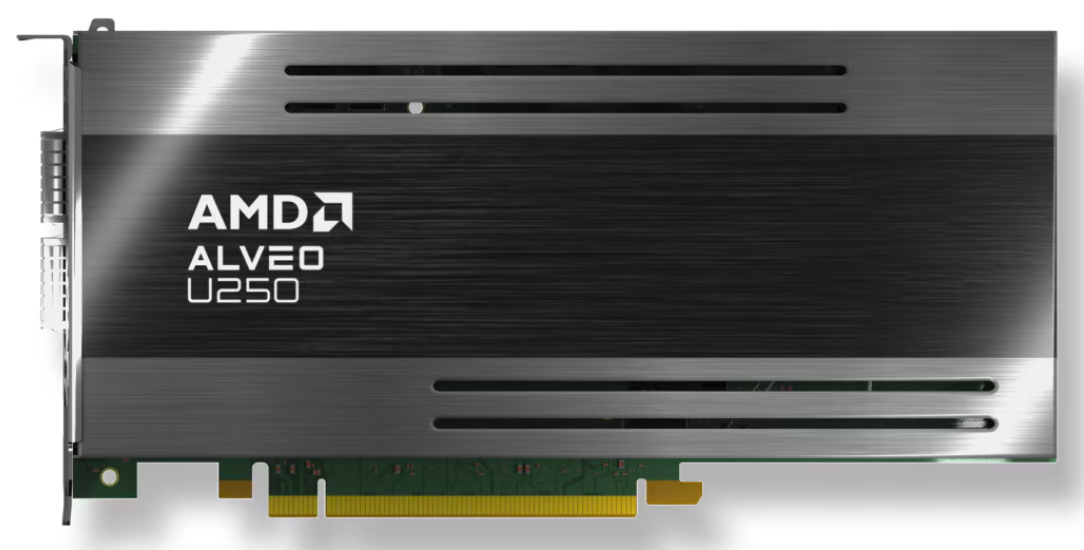
\includegraphics[width=0.7\textwidth]{figures/chapter3/alveou250.png}
  \caption{Alveo U250}
  \label{fig:alveou250}
\end{figure}

Kάρτες επιτάχυνσης όπως η AMD Alveo που παρέχει αντίστοιχα το AWS έχουν σχεδιαστεί με γνώμονα τα κέντρα δεδομένων για να ανταποκρίνονται στις συνεχώς μεταβαλλόμενες ανάγκες των σύγχρωνων εφαρμογών 
προσφέροντας έως και 90 φορές αύξηση απόδοσης σε σχέση με τους επεξεργαστές (CPUs). Συγκεκριμένα χρησιμοποιούνται για κοινές εργασίες, όπως η μηχανική μάθηση,
η μετατροπή βίντεο και η αναζήτηση και ανάλυση βάσεων δεδομένων. Με την εξέλιξη των σύνθετων αλγορίθμων να είναι ταχύτερη από τους γενιές υλικού IC,
οι συσκευές σταθερής λειτουργίας όπως οι GPU και τα ASIC δεν μπορούν να ακολουθήσουν τον ρυθμό.


Το εργαλείο ανάπτυξης εφαρμογών της AMD \textbf{Vitis και το Machine Learning Suite} παρέχουν τα απαραίτητα εργαλεία για τους προγραμματιστές ώστε να φέρουν διαφοροποιημένες εφαρμογές στην αγορά.

Στο παρακάτω διάγραμμα παρουσιάζεται μία συγκριση μεταξύ CPU, GPU(Tesla V100) και U200 στο Azure στο οποίο διαφαίνεται η υψηλή επιτάχυνση ενός Deen Neural Network νευρωνικού δικτύου για ανάλυση εικόνων με 
(αποκαλούμενο και με την ονομασία Inception Net) σε σχέση με τους άλλους επεξεργαστές. Το ίδιο φαίνεται και στην δεύτερη φωτογραφία όπου ο χρόνος ανάλυσης είναι μικρότερος σε σχέση με την GPU για ενα CNN συνδυασμένο με Bidirectional LSTM.

\begin{figure}[h!]
  \centering
  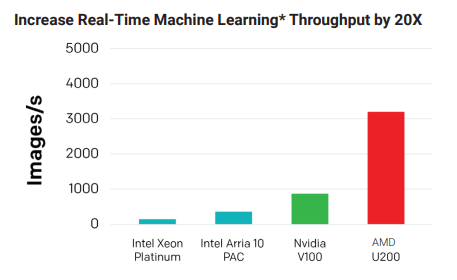
\includegraphics[width=0.7\textwidth]{figures/chapter3/u200_throughput_comparison.png}
  \caption{Alveo u200 Throughput Comparison}
  \label{fig:u200_throughput_comparison}
\end{figure}
\begin{figure}[h!]
  \centering
  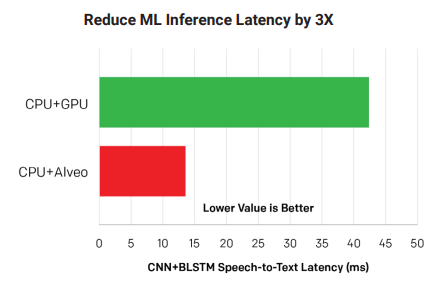
\includegraphics[width=0.7\textwidth]{figures/chapter3/cnn_u200.png}
  \caption{Alveo u200 Throughput Comparison 2}
  \label{fig:cnn_u200.png}
\end{figure}

Όπως είπαμε προηγουμένως και ο μεγαλύτερος μέχρι στιγμής πάροχος infrastracture η Amazon Web Services (AWS), προσφέρει ισχυρές λύσεις FPGA πλέον μέσω των \textbf{EC2 F2 instances},
τα οποία είναι σχεδιασμένα για ανάπτυξη και υλοποίηση επαναπρογραμματιζόμενου υλικού στο cloud.
Τα F2 instances αποτελούν τη \textbf{δεύτερη γενιά FPGA-powered instances} και προσφέρουν έως και 60\% καλύτερη σχέση τιμής-απόδοσης σε σύγκριση με την πρώτη γενιά F1 instances.
Τα F2 instances είναι εξοπλισμένα με έως και 8 \textbf{AMD Virtex UltraScale+ HBM VU47P} FPGAs, τα οποία διαθέτουν \textbf{16GB μνήμης υψηλού εύρους ζώνης (HBM - High Band Memory)}.
Επιπλέον, περιλαμβάνουν επεξεργαστή 3ης γενιάς AMD EPYC (Milan) με 192 vCPU, 100 Gbps δικτυακό εύρος ζώνης, 2 TiB μνήμη συστήματος, και 7.6 TiB μέσω NVMe SSD.
Η ανάπτυξη σε F2 instances είναι απλή, καθώς παρέχουν όλα τα απαραίτητα εργαλεία για ανάπτυξη, προσομοίωση, αποσφαλμάτωση και σύνθεση κώδικα επιτάχυνσης υλικού μέσω του FPGA Developer AMI.
Οι προγραμματιστές μπορούν να χρησιμοποιήσουν περιβάλλοντα ανάπτυξης για χαμηλού επιπέδου υλικό, καθώς και για ανάπτυξη λογισμικού σε C/C++ και OpenCL.
Η AWS, μέσω των F2 instances, προσφέρει μια ευέλικτη και οικονομικά αποδοτική πλατφόρμα για την ανάπτυξη και υλοποίηση εξειδικευμένων FPGA-επιταχυνόμενων λύσεων στο cloud.

\begin{figure}[h!]
  \centering
  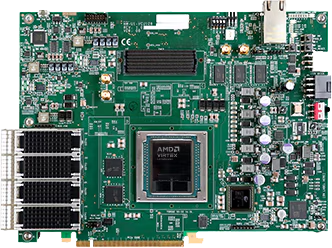
\includegraphics[width=0.4\textwidth]{figures/chapter3/aws_fpga.png}
  \caption{AMD Virtex UltraScale+ HBM VU47P on Amazon}
  \label{fig:aws_fpga.png}
\end{figure}

\section{Δομικά Στοιχεία FPGA}
\label{sec:fpga_building_blocks}

TODO: Να γράψω για τα δομικά στοιχεία των FPGA,
- CLBs (Configurable Logic Blocks)
- DSP Slices
- BRAM (Block RAM)
- Clock Management
- Configuration Memory
https://digilent.com/blog/structure-of-an-fpga/?srsltid=AfmBOoqiel0G33eFjSXgiICQtpLf8xmEr5Y3WUDmdNXS6MicKzivStvE

Οπως περιγράψαμε προηγουμένως τα σύγχρονα FPGA μπορούν να εκτελέσουν ταχύτατους υπολογισμούς και να υλοποιήσουν πολύπλοκες λειτουργίες
και για να επιτύχουν αυτή την απόδοση βασίζονται σε μια σειρά από δομικά στοιχεία που συνεργάζονται αρμονικά τα οποία θα αναλύσουμε σε αυτό το κεφάλαιο.

Τα βασικά δομικά στοιχεία των FPGA περιλαμβάνουν:
\begin{enumerate}
  \item \textbf{LUTs:} Lookup Tables
  \item \textbf{FFs:} Flip Flops
  \item \textbf{Connections:} Διασυνδέσεις/Traces μεταξύ των στοιχείων του FPGA
  \item \textbf{I/O:} Input/Output Pads/Ports
\end{enumerate}

\subsection{Lookup Tables (LUTs)}

Τα Lookup Tables (LUTs) είναι τα πιο βασικά δομικά στοιχεία των FPGA και χρησιμοποιούνται για την υλοποίηση λογικών συναρτήσεων.
Ουσιαστικά κάθε LUT είναι ένας πίνακας αληθείας που αποθηκεύει τις εξόδους απο ένα εύρος δίαφορων τιμών εισόδων.
Αυτή η διαδικασία συναντάται συνήθως σε υλοποιήσεις προγραμμάτων που εκτελούνται μικροεπεξεργαστές και μικροελενκτές ωστε να επιτυγχανονται γρηγορότεροι υπολογισμοί
αλλά και να μήν γινονται συνέχεις υπολογισμοί που γνωρίζουμε οτι θα χρειαστούν εκ των προτέρων.
Αυτό συναντάται πολύ συχνά σε safety-critical εφαρμογές , όπως σε αεροδιαστημικές εφαρμογές, ιατρικές συσκευές και σαφώς στην αυτοκινητοβιομηχανία,
όπου η ταχύτητα και η αξιοπιστία των υπολογισμών είναι ζωτικής σημασίας.
Ωστόσο αυτή η μορφή των Lookup Tables την οποία μόλις περιέγραψα γίνεται σε επίπεδο λογισμικού και όχι σε επίπεδο υλικού.
Τα FPGA πηγαίνουν τα Lookup Tables στο επόμενο επίπεδο καθώς \textbf{η υλοποίηση τους γίνεται σε επίπεδο υλικού} και συνεπώς η ταχύτητα των υπολογισμών είναι πολύ μεγαλύτερη!

\begin{figure}[h!]
  \centering
  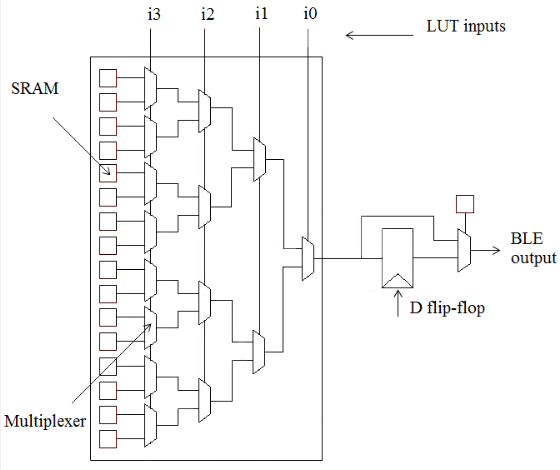
\includegraphics[width=0.7\textwidth]{figures/chapter3/lut_diagram.png}
  \caption{Διάγραμμα δομής και λειτουργίας ενός 4-input LUT}
  \label{fig:lut_diagram}
\end{figure}

Ένα LUT (Look-Up Table) αποτελεί το βασικό δομικό στοιχείο ενός FPGA και είναι ικανό να υλοποιήσει οποιαδήποτε λογική συνάρτηση \(N\) Boolean μεταβλητών. Ουσιαστικά, το LUT λειτουργεί ως ένας πίνακας αληθείας, όπου κάθε δυνατός συνδυασμός εισόδων αντιστοιχεί σε μια συγκεκριμένη έξοδο. Το μέγεθος του πίνακα αληθείας καθορίζεται από τον αριθμό των εισόδων \(N\), με τον συνολικό αριθμό θέσεων μνήμης να δίνεται από τον τύπο:

\[
\text{Αριθμός θέσεων μνήμης} = 2^N
\]

Αυτό σημαίνει ότι το LUT μπορεί να υλοποιήσει συνολικά:
\[
\text{Αριθμός δυνατών συναρτήσεων} = 2^{N^N}
\]


Για παράδειγμα, σε ένα τυπικό FPGA της Xilinx, η τιμή του \(N\) είναι συνήθως 6, επιτρέποντας στο LUT να υλοποιήσει οποιαδήποτε συνάρτηση 6 εισόδων.

Η υλοποίηση ενός LUT σε υλικό μπορεί να θεωρηθεί ως μια συλλογή κυττάρων μνήμης που συνδέονται με ένα σύνολο πολυπλεκτών (multiplexers). Οι είσοδοι του LUT λειτουργούν ως bits επιλογής στους πολυπλέκτες, καθορίζοντας ποια τιμή μνήμης θα εμφανιστεί στην έξοδο σε κάθε χρονική στιγμή. Αυτή η προσέγγιση επιτρέπει στο LUT να χρησιμοποιείται τόσο ως υπολογιστική μονάδα λογικών συναρτήσεων όσο και ως στοιχείο αποθήκευσης δεδομένων.

\subsection{Flip-Flops (FFs)}

Τα Flip-Flops (FFs) αποτελούν το βασικό στοιχείο αποθήκευσης δεδομένων στην αρχιτεκτονική ενός FPGA. Ένα flip-flop είναι ένας απλός καταχωρητής που μπορεί να αποθηκεύσει ένα bit πληροφορίας και χρησιμοποιείται για τη διατήρηση της κατάστασης ενός σήματος μεταξύ κύκλων ρολογιού. Σε κάθε κύκλο του ρολογιού, το flip-flop ενημερώνει την τιμή του με βάση την είσοδό του, επιτρέποντας έτσι τη δημιουργία ακολουθιακών κυκλωμάτων και την υλοποίηση χρονισμένων λειτουργιών.

Στα FPGA, \textbf{κάθε LUT συνήθως συνοδεύεται από ένα ή περισσότερα flip-flops}, ώστε το αποτέλεσμα της λογικής λειτουργίας να μπορεί να αποθηκευτεί και να χρησιμοποιηθεί σε επόμενους κύκλους. Αυτός ο συνδυασμός LUT και flip-flop είναι το θεμέλιο για τη δημιουργία πιο σύνθετων δομών, όπως καταχωρητές, μετρητές, καταχωρητές ολίσθησης (shift registers) και finite state machines (FSM).

Η χρήση flip-flops είναι απαραίτητη για την υλοποίηση ακολουθιακών κυκλωμάτων, όπου η έξοδος εξαρτάται όχι μόνο από τις τρέχουσες εισόδους αλλά και από προηγούμενες καταστάσεις του συστήματος. Τα flip-flops επιτρέπουν τον συγχρονισμό των δεδομένων με το ρολόι του συστήματος, διασφαλίζοντας αξιόπιστη λειτουργία και σωστή αλληλουχία των γεγονότων.
Η βασική δομή ενός flip-flop περιλαμβάνει τις ακόλουθες εισόδους και εξόδους:
\begin{itemize}
  \item \textbf{Data Input (D):} Η τιμή που πρόκειται να αποθηκευτεί.
  \item \textbf{Clock Input (CLK):} Ο παλμός του ρολογιού που συγχρονίζει τη λειτουργία του flip-flop.
  \item \textbf{Clock Enable (CE):} Όταν είναι ενεργό, επιτρέπει την ενημέρωση της αποθηκευμένης τιμής.
  \item \textbf{Reset (R):} Επαναφέρει την έξοδο του flip-flop σε προκαθορισμένη τιμή (συνήθως μηδέν).
  \item \textbf{Data Output (Q):} Η τρέχουσα αποθηκευμένη τιμή.
\end{itemize}

\begin{figure}[h!]
  \centering
  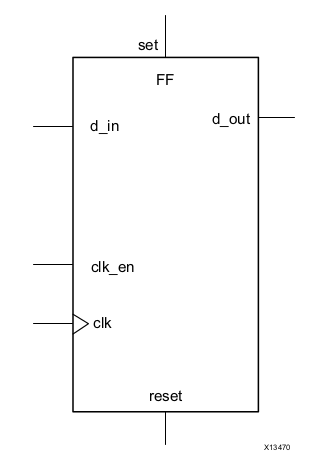
\includegraphics[width=0.3\textwidth]{figures/chapter3/flip_flop_schema.png}
  \caption{Block σχεδίασης Flip-Flop (FF)}
  \label{fig:flipflop_schema}
\end{figure}

Κατά τη διάρκεια της λειτουργίας, το flip-flop ενημερώνει την έξοδό του με την τιμή της εισόδου δεδομένων σε κάθε παλμό του ρολογιού, εφόσον το clock enable είναι ενεργό. Αν το clock enable δεν είναι ενεργό, το flip-flop διατηρεί την προηγούμενη τιμή του, επιτρέποντας έτσι την προσωρινή αποθήκευση δεδομένων για περισσότερους από έναν κύκλους ρολογιού. Η είσοδος reset χρησιμοποιείται για την αρχικοποίηση ή την επαναφορά του flip-flop σε γνωστή κατάσταση.

Η συνδυασμένη χρήση LUTs και flip-flops στα FPGA επιτρέπει την υλοποίηση τόσο συνδυαστικών όσο και ακολουθιακών λογικών κυκλωμάτων, προσφέροντας ευελιξία στον σχεδιασμό πολύπλοκων ψηφιακών συστημάτων. Τα flip-flops είναι απαραίτητα για την υλοποίηση καταχωρητών, μετρητών, finite state machines (FSM), και άλλων ακολουθιακών δομών που απαιτούν αποθήκευση κατάστασης και χρονισμό.

\begin{figure}[h!]
  \centering
  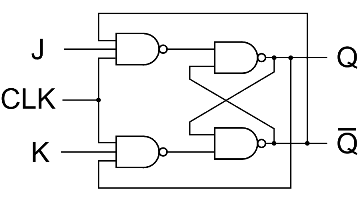
\includegraphics[width=0.5\textwidth]{figures/chapter3/flip_flop_fpga.png}
  \caption{Πύλες ενός Flip-Flop (FF)}
  \label{fig:flipflop_diagram}
\end{figure}

\subsection{Connections}

Οι διασυνδέσεις αποτελούν την ραχοκοκαλια μεταξύ των δομικών στοιχείων ενός FPGA, όπως LUTs, Flip-Flops, DSP slices και I/O blocks. Πρόκειται για προγραμματιζόμενες γραμμές μετάδοσης σήματος που επιτρέπουν τη μεταφορά δεδομένων και ελέγχου σε όλο το chip.

Οι διαδρομές (wires) και οι διακόπτες (switches) όπως \textbf{antifuse ή pass transistors} αποτελούν τους βασικούς πόρους δρομολόγησηςπου χρησιμοποιούνται για τη μεταφορά σημάτων μεταξύ block στα FPGA. Οι πόροι αυτοί οργανώνονται σε ειδικές περιοχές που ονομάζονται \textbf{routing channels}, οι οποίες έχουν σταθερό μέγεθος και περιέχουν συγκεκριμένο αριθμό διαδρομών. Ανάλογα με τον προσανατολισμό των wires, τα routing channels διακρίνονται σε οριζόντια και κάθετα.

\begin{figure}[h!]
  \centering
  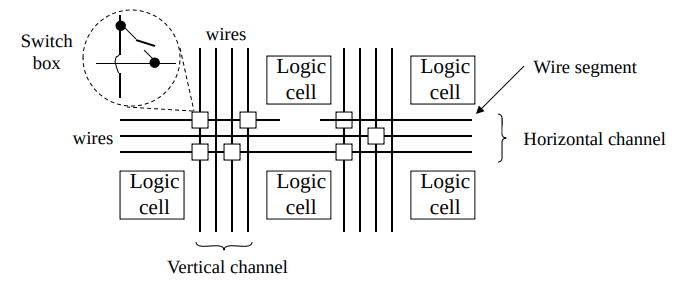
\includegraphics[width=0.8\textwidth]{figures/chapter3/interconnect.png}
  \caption{Διάγραμμα διασυνδέσεων (interconnect) σε FPGA}
  \label{fig:interconnect}
\end{figure}

Κάθε διαδρομή (track) σε ένα routing channel μπορεί να μεταφέρει ένα σήμα, και η χωρητικότητα (capacity) του καναλιού ισούται με τον αριθμό των tracks που περιέχει.

Προς το παρόν υπάρχουν δύο βασικές φιλοσοφίες σχεδίασης των διασυνδέσεων στα FPGA:
\begin{itemize}
  \item \textbf{Antifuse Technology:} Χρησιμοποιεί μόνιμες διασυνδέσεις που δημιουργούνται κατά την κατασκευή του FPGA. Αυτές οι διασυνδέσεις δεν μπορούν να επαναπρογραμματιστούν, αλλά προσφέρουν υψηλή πυκνότητα.
  \item \textbf{Pass Transistor Technology:} Χρησιμοποιεί διακόπτες που μπορούν να επαναπρογραμματιστούν, επιτρέποντας μεγαλύτερη ευελιξία στη δρομολόγηση, αλλά με αυξημένη καθυστέρηση και κατανάλωση ισχύος.
\end{itemize}

\begin{figure}[h!]
  \centering
  \begin{minipage}{0.48\textwidth}
    \centering
    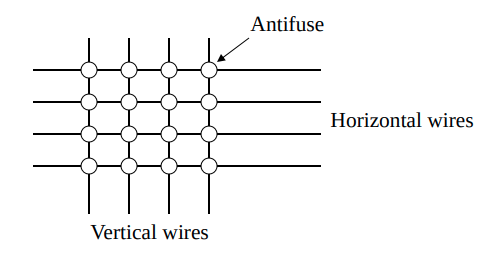
\includegraphics[width=\textwidth]{figures/chapter3/antifuse.png}
    \caption{Διασύνδεση Antifuse}
    \label{fig:antifuse}
  \end{minipage}\hfill
  \begin{minipage}{0.48\textwidth}
    \centering
    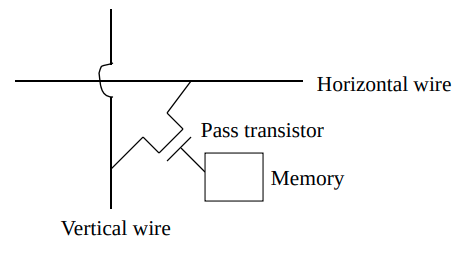
\includegraphics[width=\textwidth]{figures/chapter3/pass_transistor.png}
    \caption{Διασύνδεση Pass Transistor}
    \label{fig:pass_transistor}
  \end{minipage}
\end{figure}

Στα FPGA η antifuse τεχνολογία, μπορεί να βρίσκεται σε κάθε οριζόντια και κάθετη διαδρομής, καθώς καταλαμβάνει πολύ μικρή επιφάνεια. Αυτή η δομή ονομάζεται \textbf{fully populated} και προσφέρει υψηλή ευελιξία στη δρομολόγηση, \textbf{αλλά δεν μπορεί να επαναπρογραμματιστεί}. Επίσης προσθέτουν σημαντική παρασιτική αντίσταση και χωρητικότητα, οδηγώντας σε αυξημένη καθυστέρηση διάδοσης και κατανάλωση ισχύος.

Αντίθετα, οι διακόπτες με pass transistors και οι αντίστοιχες μνήμες καταλαμβάνουν μεγαλύτερη επιφάνεια, καθιστώντας μη ρεαλιστική την πλήρη υλοποίηση fully populated δομής. Συνήθως, αυτή η τεχνολογία προσφέρει μικρότερη ευελιξία στη δρομολόγηση, αλλά επιτρέπει επαναπρογραμματισμό.

Οι μεγαλύτερες διασυνδέσεις αποκαλούνται interconnects, οι οποίες είναι το σύνολο των προγραμματιζόμενων διασυνδέσεων που επιτρέπουν την επικοινωνία μεταξύ διαφορετικών logic blocks, memory blocks και I/O.

Οι διασυνδέσεις διακρίνονται σε:
\begin{itemize}
  \item \textbf{Programmable Switch Matrices:} Δικτυώματα διακοπτών που επιτρέπουν την επιλογή διαδρομής μεταξύ πολλών πιθανών συνδέσεων.
  \item \textbf{Global, Regional και Local Interconnects:} Διαφορετικά επίπεδα διασύνδεσης για σύνδεση μακρινών ή γειτονικών blocks, αντίστοιχα.
  \item \textbf{Long Lines και Short Lines:} Χρησιμοποιούνται για μεταφορά σήματος σε μεγάλες ή μικρές αποστάσεις εντός του FPGA.
\end{itemize}

Η αρχιτεκτονική των interconnects επηρεάζει άμεσα την απόδοση του FPGA, καθώς η καθυστέρηση και η κατανάλωση ισχύος εξαρτώνται από το πώς δρομολογούνται τα σήματα. Οι σύγχρονες αρχιτεκτονικές FPGA διαθέτουν εξελιγμένα δίκτυα διασύνδεσης που υποστηρίζουν ταυτόχρονη επικοινωνία μεταξύ πολλών blocks, επιτρέποντας υψηλό βαθμό παραλληλισμού.

Επιπλέον, τα interconnects διαδραματίζουν σημαντικό ρόλο στην επικοινωνία μεταξύ ενσωματωμένων επεξεργαστών (π.χ. ARM cores) και της προγραμματιζόμενης λογικής, μέσω ειδικών διαύλων όπως AXI, Avalon ή custom high-speed fabrics. Η βελτιστοποίηση των interconnects είναι απαραίτητη για εφαρμογές που απαιτούν υψηλό throughput, όπως machine learning, επεξεργασία σήματος και δικτυακές εφαρμογές.

\subsection{Input/Output (I/O) Blocks}

Τα I/O Blocks (Input/Output Blocks) αποτελούν το σημείο σύνδεσης μεταξύ του εσωτερικού κυκλώματος του FPGA και του εξωτερικού περιβάλλοντος. Κάθε I/O block μπορεί να διαμορφωθεί ως είσοδος, έξοδος ή αμφίδρομη θύρα, επιτρέποντας ευέλικτη επικοινωνία με άλλα ψηφιακά ή αναλογικά συστήματα.

Συνήθως, κάθε I/O block περιλαμβάνει D flip-flops για την καταχώρηση των σημάτων εισόδου και εξόδου, προσφέροντας συγχρονισμό και αξιόπιστη μεταφορά δεδομένων. Αυτό επιτρέπει την αποφυγή μεταβατικών φαινομένων και τη σωστή χρονική ευθυγράμμιση των σημάτων με το ρολόι του συστήματος.

Τα I/O blocks υποστηρίζουν διάφορα πρότυπα τάσης και πρωτόκολλα επικοινωνίας, ενώ συχνά διαθέτουν δυνατότητες όπως pull-up/pull-down resistors, προσαρμογή ταχύτητας (slew rate), και προστασία από ηλεκτροστατική εκφόρτιση (ESD).

Η σωστή διαμόρφωση των I/O blocks είναι κρίσιμη για την αξιόπιστη λειτουργία του FPGA, ειδικά σε εφαρμογές υψηλής ταχύτητας ή απαιτητικής ηλεκτρομαγνητικής συμβατότητας.

\begin{figure}[h!]
  \centering
  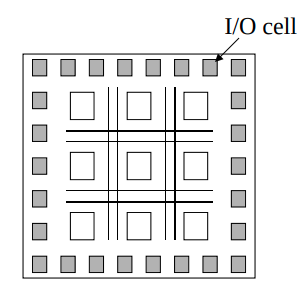
\includegraphics[width=0.6\textwidth]{figures/chapter3/io_block.png}
  \caption{Δομή I/O Block σε FPGA}
  \label{fig:io_block}
\end{figure}

\subsection{Configurable Logic Blocks (CLBs)}
Οταν ενώσουμε αυτά τα βασικά δομικά στοιχεία μπορούμε να δημιουργήσουμε ανώτερα μπλοκ που χρησιμοποιούνται για την υλοποίηση πιο σύνθετων λειτουργιών.
Ενα απο αυτά τα μπλοκ είναι τα \textbf{Configurable Logic Blocks (CLBs)}.

Τα Configurable Logic Blocks (CLBs) είναι ο βασικός επαναλαμβανόμενος πόρος λογικής σε ένα FPGA. Όταν συνδέονται μεταξύ τους μέσω δρομολόγησης, μπορούν να υλοποιήσουν
σύνθετες λογικές συναρτήσεις, δομές μνήμης καθώς και να συγχρονίσουν την εκτέλεση κώδικα στο σύστημα.

Συνήθως ένα CLB περιλαμβάνει πολλαπλά LUTs, flip-flops, πολυπλέκτες. Τα βασικά του στοιχεία είναι:
\begin{itemize}
  \item \textbf{Flip-Flop (FF)}
  \item \textbf{Look-Up Table (LUT)}
  \item \textbf{Multiplexer (MUX)}
\end{itemize}

\begin{figure}[h!]
  \centering
  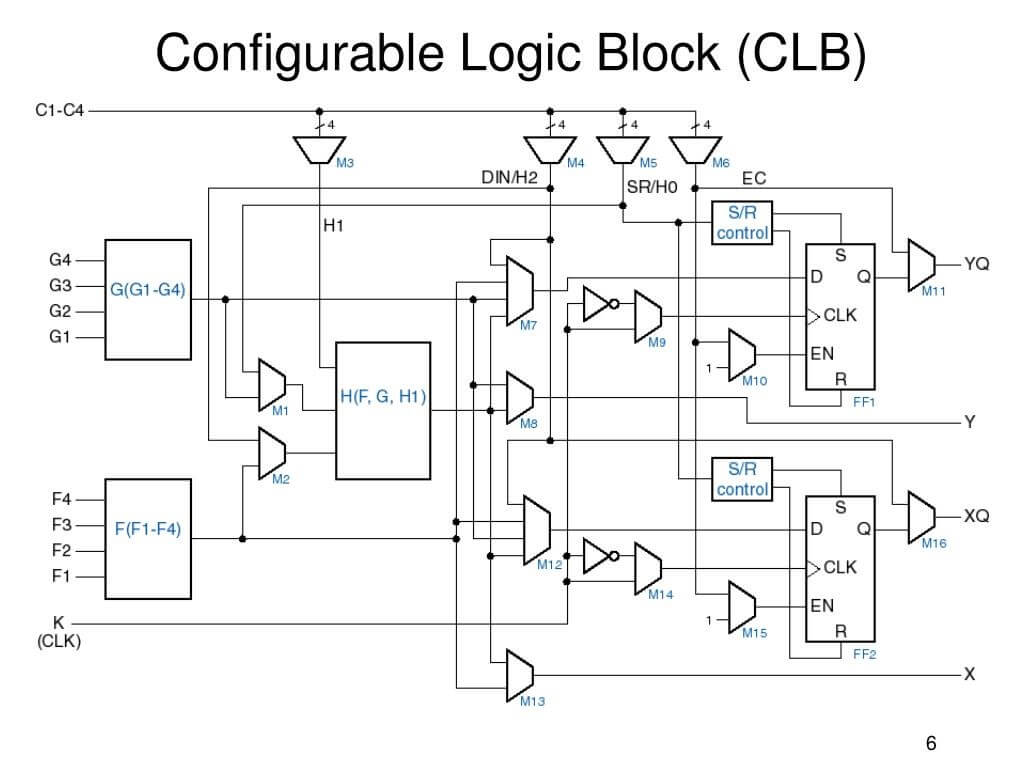
\includegraphics[width=1.0\textwidth]{figures/chapter3/clb_block.png}
  \caption{CLB Block σε FPGA}
  \label{fig:clb_block}
\end{figure}

Στις σύγχρονες αρχιτεκτονικές, κάθε CLB αποτελείται από πολλαπλά \emph{slices}, με κάθε slice να συνδυάζει 8 input LUTs, 16 FFs, ενα δίκτυο carry logic και 3 είδη πολυπλεκτών MUX
προσφέροντας υψηλό βαθμό παραλληλισμού και πυκνότητα λογικής. Με σωστή αξιοποίηση των LUTs ως μνήμη ή SRLs και με χρήση των carry chains, τα CLBs επιτυγχάνουν υψηλές συχνότητες λειτουργίας και αποδοτική χρήση πόρων.

\subsubsection{Carry Chain στα CLBs}

Στα σύγχρονα FPGA κάθε slice διαθέτει ειδική «γρήγορη» αλυσίδα κρατουμένου που υλοποιείται με αφιερωμένους πολυπλέκτες και πύλες XOR (π.χ. MUXCY/XORCY). Η αλυσίδα αυτή έχει ύψος 4 bit ανά slice και συνδέει κατακόρυφα τις στήλες από slices, ώστε να υλοποιούνται πολύ γρήγορα αθροιστές, αφαιρέτες και στάδια μεταφοράς σε πολλαπλασιαστές.

Η βασική εξίσωση προώθησης κρατουμένου ορίζεται μέσω σημάτων propagate και generate:
\[
p_i = a_i \oplus b_i,\quad g_i = a_i \cdot b_i
\]
\[
c_{i+1} = g_i \lor (p_i \cdot c_i), \qquad s_i = p_i \oplus c_i
\]

Ιδιότητες και χρήσεις:
\begin{itemize}
  \item 4-bit ύψος ανά slice, με κατακόρυφη διασύνδεση για αλυσίδωση πολλών slices χωρίς βαριά δρομολόγηση.
  \item Πρόσθεση N-bit με πολύ μικρή καθυστέρηση ανά bit (χαρτογράφηση σε dedicated carry hardware).
  \item Αφαίρεση μέσω συμπληρώματος ως \(A + \overline{B} + 1\) στην ίδια αλυσίδα κρατουμένου.
  \item Ταχύς συγκριτής μέτρου (έλεγχος carry-out) και μετρητές.
  \item Χρήση σε πολλαπλασιασμό μέσα σε δένδρα άθροισης μερικών (carry save | propagate στάδια).
\end{itemize}

\subsection{Digital Signal Processing Slices (DSP)}

Τα FPGAs είναι ιδιαίτερα αποδοτικά για εφαρμογές ψηφιακής επεξεργασίας σήματος (DSP), 
επειδή υλοποιούν προσαρμοσμένους, πλήρως παράλληλους αλγορίθμους. 
Οι εφαρμογές DSP χρησιμοποιούν εκτενώς δυαδικούς πολλαπλασιαστές και συσσωρευτές (MAC)
που υλοποιούνται βέλτιστα σε αφιερωμένα DSP slices.
Όλες οι FPGA συσκευές διαθέτουν πολλα, πλήρως custom και χαμηλής κατανάλωσης DSP slices,
συνδυάζοντας υψηλή ταχύτητα με μικρό αποτύπωμα, ενώ διατηρούν ευελιξία στον σχεδιασμό.
Επιπλέον, οι DSP slices επιταχύνουν και μη‑DSP εργασίες, όπως δυναμικούς shifters,
γεννήτριες διευθύνσεων μνήμης, ευρείς πολυπλέκτες και memory‑mapped I/O καταχωρητές.

\begin{figure}[h!]
  \centering
  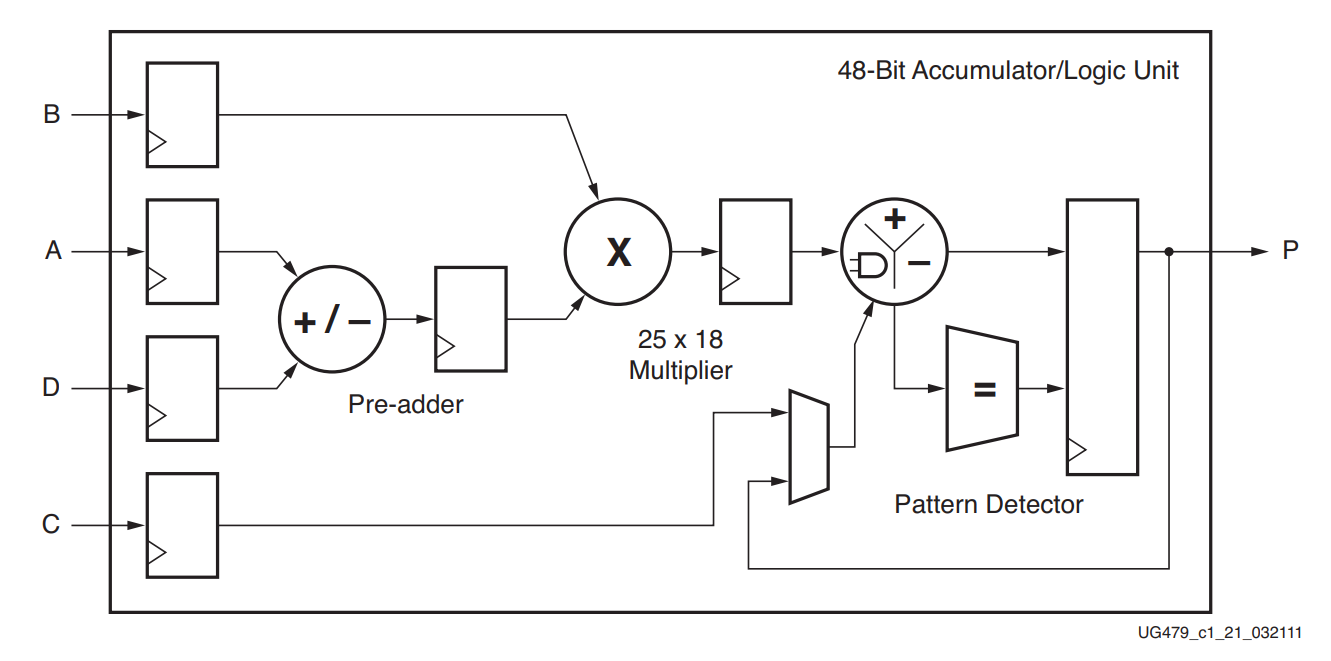
\includegraphics[width=1.0\textwidth]{figures/chapter3/dsp_block.png}
  \caption{DSP Block σε FPGA - DSP48E1}
  \label{fig:dsp_block}
\end{figure}


Κύρια χαρακτηριστικά των DSP slices:
\begin{itemize}
  \item \textbf{Πολλαπλασιαστής 25×18 σε two’s-complement} με δυναμική παρακαμψη για μείωση καθυστέρησης όταν ο πολλαπλασιασμός παρακάμπτεται.
  \item \textbf{Συσσωρευτής 48-bit (ACC)} που μπορεί να διαμορφωθεί και ως σύγχρονος up/down counter.
  \item \textbf{Προ-αθροιστής εξοικονόμησης ισχύος (pre-adder)}, ιδανικός για συμμετρικά FIR φίλτρα, μειώνοντας τον αριθμό απαιτούμενων DSP slices.
  \item \textbf{SIMD μονάδα αριθμητικής}:
    \begin{itemize}
      \item Διπλό 24-bit (\emph{dual 24-bit}) add/sub/accumulate
      \item Τετραπλό 12-bit (\emph{quad 12-bit}) add/sub/accumulate
    \end{itemize}
  \item \textbf{Προαιρετική μονάδα λογικής} που μπορεί να υλοποιήσει μία από 10 λογικές συναρτήσεις επί των δύο τελεστέων.
  \item \textbf{Ανιχνευτής προτύπων (pattern detector)} με υγκλίνουσα ή συμμετρική στρογγυλοποίηση για ελεγχόμενη στρογγυλοποίηση
  αλλά και λειτουργίες λογικής έως 96-bit πλάτου όταν χρησιμοποιείται σε συνδυασμό με τη μονάδα λογικής.
  \item \textbf{Προηγμένες δυνατότητες}: προαιρετικό pipelining σε πολλαπλά στάδια και αφιερωμένοι δίαυλοι διασύνδεσης.
\end{itemize}

\subsection{Block Random Access Memory (BRAM)}
Τα Block RAMs (BRAM) είναι ενσωματωμένες μνήμες τυχαίας προσπέλασης μέσα στο FPGA και χρησιμοποιούνται για αποθήκευση «μεγάλων» όγκων δεδομένων
σε σχέση με τις διανεμημένες μνήμες (LUT/Distributed RAM).
Αποτελούν διακριτούς πόρους καθώς κάθε συσκευή έχει πεπερασμένο αριθμό BRAM blocks (π.χ. 18/36 Kb στις AMD/Xilinx, 10/20 Kb στις Intel, 9 Kb στις Lattice)
ενώ σε νεότερες οικογένειες συνυπάρχει και \textbf{UltraRAM μεχρι και 288 Kb} για ακόμη μεγαλύτερη χωρητικότητα.

Κύρια χαρακτηριστικά:
\begin{itemize}
  \item Παραμετροποιήσιμες σε πλάτος/βάθος με trade‑off μεταξύ εύρους λέξης και αριθμού διευθύνσεων.
  \item Θύρες πρόσβασης - single‑port, simple dual‑port (ξεχωριστή ανάγνωση/εγγραφή), true dual‑port (δύο ανεξάρτητες θύρες R/W, συχνά με ανεξάρτητα ρολόγια).
  \item Πολιτικές σύγκρουσης - read‑first, write‑first, no‑change (διαθέσιμες ανά οικογένεια/primitive).
  \item Επιπρόσθετα: byte‑enable, parity/ECC
\end{itemize}

Βασικές κατηγορίες μνήμης:
\begin{itemize}
  \item BRAM: μεγάλοι πίνακες, frame buffers, FIFOs/queues, πίνακες συντελεστών/lookup, scratchpads με υψηλή πυκνότητα και χαμηλή κατανάλωση.
  \item Distributed RAM (LUT RAM): μικρές μνήμες πολύ κοντά στη λογική με εξαιρετικά χαμηλή καθυστέρηση.
  \item UltraRAM: πολύ μεγάλες on‑chip μνήμες με υψηλή απόδοση, χρήσιμες για βάθια buffers.
  \item Off‑chip (SRAM/DDR/HBM/SD): όταν η απαίτηση χωρητικότητας ξεπερνά τους on‑chip πόρους.
\end{itemize}

Ενδεικτικές χρήσεις:
\begin{itemize}
  \item Πίνακες συντελεστών φίλτρων/DSP, εικόνες/tiles, lookup tables μεγάλης κλίμακας.
  \item Σειρές/στοίβες FIFOs/BRAM με dual‑port για ανεξάρτητους παραγωγούς/καταναλωτές.
  \item Μνήμη για επιταχυντές HLS με παραλληλοποίηση για αυξημένο throughput.
\end{itemize}


\section{Εργαλεία Εξομοίωσης και Επαλήθευσης}


Τα σύγχρονα εργαλεία εξομοίωσης και επαλήθευσης είναι απαραίτητα για την αποτελεσματική ανάπτυξη εφαρμογών FPGA.
Αυτά τα εργαλεία επιτρέπουν στους μηχανικούς να επαληθεύουν τη λειτουργικότητα των σχεδίων τους πριν την υλοποίηση στο πραγματικό υλικό, εξοικονομώντας χρόνο και πόρους.
Υπάρχουν ποικίλα εργαλεία που διατίθενται τόσο από τη Xilinx (πλέον AMD) όσο και από την Intel (πρώην Altera), τους δύο κύριους κατασκευαστές FPGA.

\subsection{Εργαλεία Κατασκευαστών}

\subsubsection{Xilinx (AMD) Εργαλεία}
\begin{itemize}
  \item \textbf{Vivado HL Design Edition}: Για FPGAs UltraScale, UltraScale+ και 7 Series. Βελτιστοποιημένο για την υποστήριξη προηγμένων χαρακτηριστικών στις νεότερες γενιές FPGA και SoC.
  
  \item \textbf{ISE Design Suite}: Για παλαιότερες συσκευές όπως Spartan-6, Virtex-6, CoolRunner και προηγούμενες γενιές. Υποστηρίζει παλαιότερες γενιές συσκευών.
  
  \item \textbf{Vivado HL WebPACK Edition}: Δωρεάν έκδοση χωρίς άδεια, με περιορισμένη υποστήριξη συσκευών και λειτουργιών.
  
  \item \textbf{SDAccel Environment}: Περιβάλλον ανάπτυξης για OpenCL.
  
  \item \textbf{SDSoC Environment}: Ολοκληρωμένη σουίτα εργαλείων για ανάπτυξη ενσωματωμένου λογισμικού σε SoC.
  
  \item \textbf{Software Development Kit}: Ολοκληρωμένο πακέτο ανάπτυξης για ανάπτυξη και αποσφαλμάτωση κώδικα για SoC.
  
  \item \textbf{System Generator for DSP}: Εργαλείο σχεδίασης DSP για εφαρμογές ψηφιακής επεξεργασίας σήματος.
  
  \item \textbf{Vivado High-Level Synthesis}: Εργαλείο σύνθεσης υψηλού επιπέδου που δέχεται μη χρονισμένο κώδικα λογισμικού ως είσοδο και παράγει κώδικα επιπέδου μεταφοράς καταχωρητών για FPGA.
  Οπως περιγράψε και πολλές φορες προηγουμένως αυτο θα είναι το εργαλείο που θα χρησιμοποιήσουμε για την υλοποίηση μας.
\end{itemize}

\subsubsection{Intel Εργαλεία}
\begin{itemize}
  \item \textbf{Intel Quartus Prime Pro Edition}: Για Stratix 10, Arria 10, Cyclone 10 GX. Βελτιστοποιημένο για την υποστήριξη προηγμένων χαρακτηριστικών στις νέες γενιές FPGA.
  
  \item \textbf{Intel Quartus Prime Standard Edition}: Για Stratix IV/V, σειρά Arria, Cyclone IV/V, Cyclone 10 LP, και σειρά MAX. Υποστηρίζει παλαιότερες γενιές συσκευών.
  
  \item \textbf{Intel Quartus Prime Lite Edition}: Δωρεάν έκδοση χωρίς άδεια, με περιορισμένη υποστήριξη συσκευών και λειτουργιών.
  
  \item \textbf{Intel FPGA SDK for OpenCL}: Περιβάλλον ανάπτυξης για OpenCL.
  
  \item \textbf{Intel SoC FPGA Embedded Development Suite}: Ολοκληρωμένη σουίτα εργαλείων για ανάπτυξη ενσωματωμένου λογισμικού σε SoC.
  
  \item \textbf{Nios II Embedded Design Suite (EDS)}: Ολοκληρωμένο πακέτο ανάπτυξης για ανάπτυξη και αποσφαλμάτωση κώδικα για SoC.
  
  \item \textbf{DSP Builder for Intel FPGAs}: Εργαλείο σχεδίασης DSP για εφαρμογές ψηφιακής επεξεργασίας σήματος.
  
  \item \textbf{Intel HLS Compiler}: Εργαλείο σύνθεσης υψηλού επιπέδου που μετατρέπει κώδικα C/C++ σε RTL για FPGAs. Πρόκειται για την αντίστοιχη εφαρμογή του Vivado HLS απο την Intel.
\end{itemize}


\subsection{Εργαλεία Προσομοίωσης}

Τα εργαλεία προσομοίωσης είναι κρίσιμα για την επαλήθευση της συμπεριφοράς των σχεδίων FPGA πριν από την πραγματική υλοποίησή τους. Τα πιο διαδεδομένα εργαλεία προσομοίωσης είναι:

\begin{itemize}
  \item \textbf{Xilinx Vivado Simulator:} Ενσωματωμένος προσομοιωτής που υποστηρίζει όλες τις λειτουργίες του Vivado Design Suite για προσομοίωση RTL.
  
  \item \textbf{ModelSim:} Ένας ευρέως χρησιμοποιούμενος προσομοιωτής που αναπτύχθηκε από τη Mentor Graphics (τώρα μέρος της Siemens) και υποστηρίζει VHDL, Verilog, SystemC ενώ έχει ενσωματωμένο built-in C debugger.
  
  \item \textbf{Intel Quartus Prime:} Το πλήρες πακέτο σχεδίασης της Intel για FPGA που διατίθεται σε τρεις εκδόσεις (Pro, Standard, και Lite). Παρέχει ολοκληρωμένα εργαλεία για σχεδίαση, ανάλυση και σύνθεση, με υποστήριξη για τις οικογένειες FPGA της Intel. Περιλαμβάνει:
    \begin{itemize}
      \item TimeQuest Timing Analyzer για ανάλυση και βελτιστοποίηση χρονισμού
      \item Power Analyzer για ανάλυση κατανάλωσης ισχύος
    \end{itemize}
  
    \item \textbf{VCS:} Ένας υψηλής απόδοσης προσομοιωτής από τη Synopsys που χρησιμοποιείται για επαλήθευση σχεδιασμών ASIC και FPGA. Προσφέρει τα εξής πλεονεκτήματα:
      \begin{itemize}
        \item Υπερταχεία τεχνολογία προσομοίωσης με πλήρως παράλληλη αρχιτεκτονική που επιταχύνει την προσομοίωση απο 3-5 φορές
        \item Υποστήριξη για SystemVerilog, VHDL, SystemC, Verilog, OpenVera, και μικτή γλώσσα HDL
        \item Ολοκληρωμένη υποστήριξη για μεθοδολογίες επαλήθευσης Accellera UVM (Universal Verification Methodology), VMM (Verification Methodology Manual) και  OVM μεθοδολογίες.
        \item Παρέχει την τεχνολογία Native Testbench (NTB) που επιτρέπει την ενσωμάτωση κώδικα C/C++ στην προσομοίωση
        \item Υποστηρίζει τεχνικές power-aware προσομοίωσης για εκτίμηση κατανάλωσης ισχύος
        \item Διαθέτει προηγμένα εργαλεία αποσφαλμάτωσης και ανάλυσης κάλυψης (coverage analysis)
      \end{itemize}

      \begin{figure}[h!]
        \centering
        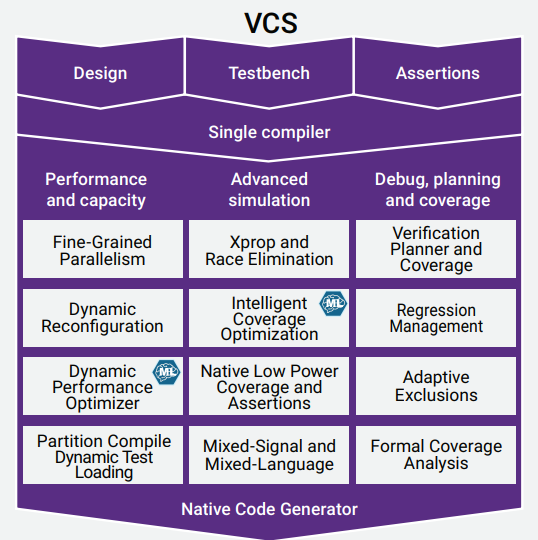
\includegraphics[width=0.8\textwidth]{figures/chapter3/vcs_software.png}
        \caption{VCS Solution}
        \label{fig:vcs_software}
      \end{figure}


  \item \textbf{Verilator:} Ένας προσομοιωτής ανοιχτού κώδικα για Verilog/SystemVerilog που μετατρέπει τον κώδικα σε βελτιστοποιημένη C++ ή SystemC για εξαιρετικά γρήγορη προσομοίωση. Το Verilator προσφέρει:
    \begin{itemize}
      \item Εξαιρετικά υψηλή απόδοση (10-100 φορές ταχύτερο από άλλους προσομοιωτές)
      \item Εκτεταμένη υποστήριξη για IEEE-1800 SystemVerilog
      \item Δυνατότητα αλληλεπίδρασης με κώδικα C++/SystemC
      \item Πλήρης υποστήριξη για 4-state προσομοίωση (X/Z)
      \item Εργαλεία στατικής ανάλυσης και lint για αυτόματο εντοπισμό σφαλμάτων στον κώδικα
      \item Υποστήριξη για multi-threading που επιτρέπει την αξιοποίηση πολλαπλών πυρήνων επεξεργαστή
      \item Ανάλυση κάλυψης κώδικα (code coverage), συμπεριλαμβανομένης κάλυψης γραμμών, μπλοκ και toggle
      \item Δημιουργία waveforms για αποσφαλμάτωση σε μορφή VCD/FST
      \item Διαθέσιμο σε πολλές πλατφόρμες (Linux, Windows, macOS)
      \item Χρησιμοποιείται ευρέως σε βιομηχανικά έργα, όπως τα RISC-V cores, OpenPiton και αρχιτεκτονικές BOOM
    \end{itemize}
\end{itemize}

\subsection{Εργαλεία Σύνθεσης}

Τα εργαλεία σύνθεσης μετατρέπουν τον κώδικα HDL σε μια αναπαράσταση netlists που μπορεί να υλοποιηθεί στο FPGA:

\begin{itemize}
  \item \textbf{Vivado Synthesis:} Το κύριο εργαλείο σύνθεσης της Xilinx για τα FPGAs UltraScale και 7-Series.
  
  \item \textbf{Intel Quartus Prime Synthesis:} Το αντίστοιχο εργαλείο σύνθεσης της Intel για τα FPGAs της.
  
  \item \textbf{Synplify Pro:} Ένα εργαλείο σύνθεσης από τη Synopsys που υποστηρίζει FPGAs διαφόρων κατασκευαστών.
\end{itemize}

\subsection{Εργαλεία Υψηλού Επιπέδου Σύνθεσης (HLS)}

Τα εργαλεία HLS επιτρέπουν στους προγραμματιστές να αναπτύσσουν εφαρμογές FPGA χρησιμοποιώντας γλώσσες υψηλού επιπέδου:

\begin{itemize}
  \item \textbf{Vitis HLS:} Το εργαλείο HLS της Xilinx που μετατρέπει κώδικα C, C++ και SystemC σε HDL.
  
  \item \textbf{Intel HLS Compiler:} Αντίστοιχο εργαλείο της Intel που μετατρέπει κώδικα C/C++ σε RTL για FPGAs.
  
  \item \textbf{Xilinx SDAccel/Vitis:} Ολοκληρωμένα περιβάλλοντα ανάπτυξης που επιτρέπουν τη χρήση OpenCL, C και C++ για την ανάπτυξη εφαρμογών επιτάχυνσης.
\end{itemize}

Αυτά τα εργαλεία εξομοίωσης και επαλήθευσης είναι ουσιώδη για τη σύγχρονη ροή σχεδίασης FPGA, επιτρέποντας στους μηχανικούς να επαληθεύσουν και να βελτιστοποιήσουν τα σχέδιά τους πριν την τελική υλοποίηση.


\section{Αρχιτεκτονική u200}

\begin{figure}[h!]
  \centering
  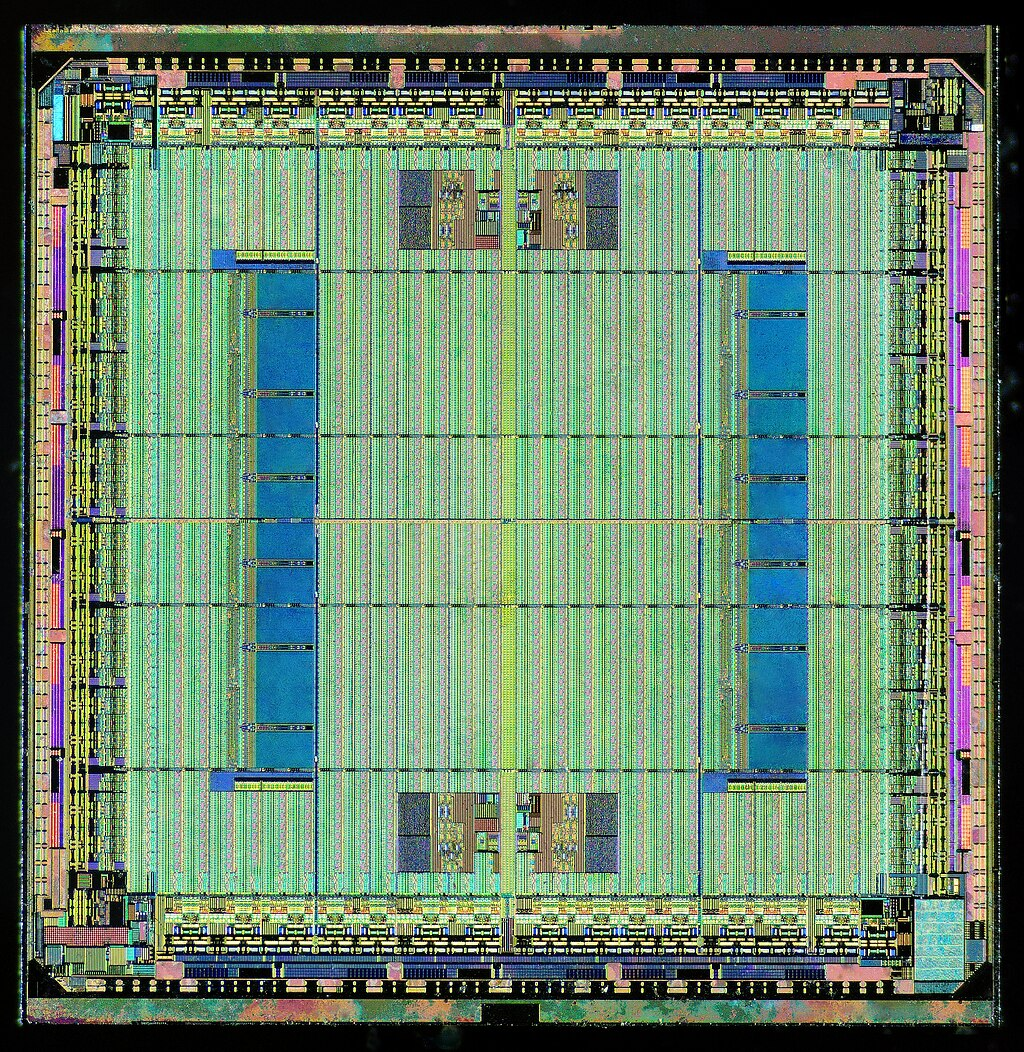
\includegraphics[width=0.8\textwidth]{figures/chapter3/fpga_core.png}
  \caption{FPGA Core}
  \label{fig:fpga_core}
\end{figure}

Η πλατφόρμα που παρέχει ο σέρβερ του ΑΠΘ διαθέτει την FPGA Alveo u200 στην οποία θα αναπτύξουμε το πρόγραμμα μας και θα εκτελέσουμε τις δοκιμές για να 
δούμε το throughput που επιτυγχάνουμε καθώς και την σύγκριση επιτάχυνσης με την CPU. Πιο συγκεκριμένα η κάρτα επιτάχυνσης Alveo u200 περιέχει:

\begin{table}[h!]
  \centering
  \begin{tabular}{|l|l|}
    \hline
    Μοντέλο και Virtex UltraScale+ XCU200-2FSGD2104E FPGA \\
    \hline
    Μνήμη και 4x16 GB DDR4, 2400 MT/s \\
    \hline
    Τύπος Μνήμης και x4/x8 unregistered dual inline memory module (UDIMM) \\
    \hline
    Διεπαφή SPI και 1 gigabit (Gb) Quad Serial Peripheral Interface (SPI) flash memory \\
    \hline
    Διεπαφή PCI και 16 δίοδοι PCI Express \\
    \hline
    Διεπαφή UART και USB-to-UART FT4232HQ bridge with Micro-AB USB connector \\
    \hline
    Διεπαφή I2C και Διαθέτει I2C \\
    \hline
    Tranceiver και Δυο κοννέκτορες QSFP28 100G \\
    \hline
    Flashing και Micro-AB universal serial bus (USB) JTAG configuration port \\
    \hline
    Power Supply και 65W PCIe, 150W PCIe 110A max, 225W 160A max \\
    \hline
  \end{tabular}
  \caption{Χαρακτηριστικά της FPGA Alveo u200}
  \label{tab:alveo_u200_specs}
\end{table}

Key Features:
Hardware: 16nm FinFET, 1.2M LUTs, 9,216 DSP slices, 64GB HBM2.
Use Cases: Data center acceleration (e.g., database search, financial modeling).
Comparison: Contrast with other Alveo cards (e.g., U250, U280) or Intel FPGAs.
References: Xilinx Alveo U200 datasheet, case studies.

\textbf{Xρειάζεται ενίσχυση: περιγραφή των υποσυστημάτων, αριθμός logic cells, memory blocks, υποστήριξη PCIe, HBM κ.λπ.}

\section{Design Flows}

Οι ροές σχεδίασης (design flows) για την ανάπτυξη εφαρμογών σε FPGA διαφέρουν ανάλογα με την πολυπλοκότητα του έργου και τις απαιτήσεις του συστήματος. 
Παραδοσιακά, οι σχεδιαστές χρησιμοποιούσαν το λεγομενο RTL Flow, το οποίο απαιτεί εξειδίκευση σε γλώσσες περιγραφής υλικού όπως η VHDL ή η Verilog. 
Αυτή η προσέγγιση προσφέρει μέγιστη ευελιξία, αλλά απαιτεί σημαντικό χρόνο και προσπάθεια αλλά και εξιξεικευμένες γνώσεις σχεδίασης hardware αλλα και 
σημαντικές γνώσεις του υλικού που χρησιμοποιείται, όπως η κατανόηση της αρχιτεκτονικής του FPGA, των χρονισμών, των περιορισμών κατανάλωσης ισχύος, 
καθώς και των εργαλείων που απαιτούνται για τη σύνθεση, την προσομοίωση και την επαλήθευση του σχεδίου. Τα βασικά βήματα του RTL Flow περιλαμβάνουν:

\begin{enumerate}
  \item  RTL Coding: Περιγραφή της λειτουργικότητας του κυκλώματος σε επίπεδο μεταφοράς δεδομένων μεταξύ καταχωρητών, χρησιμοποιώντας HDL γλώσσες όπως VHDL ή Verilog.
  \item  Simulation: Προσομοίωση του σχεδίου για την επαλήθευση της λειτουργικότητας και της συμπεριφοράς του κυκλώματος.
  \item  Synthesis: Μετατροπή του RTL κώδικα σε netlist που περιγράφει τη συνδεσμολογία λογικών πυλών.
  \item  Optimization: Βελτιστοποίηση του σχεδίου για βελτίωση της απόδοσης, μείωση κατανάλωσης ενέργειας ή ελαχιστοποίηση των χρησιμοποιούμενων πόρων.
  \item  Verification: Επαλήθευση του τελικού σχεδίου ώστε να διασφαλιστεί η συμμόρφωση με τις προδιαγραφές του συστήματος.
\end{enumerate}

Μια πιο μοντέρνα και απλοποιημένη προσέγγιση είναι το \textbf{HLx Flow}, το οποίο αξιοποιεί εργαλεία όπως το IP Integrator για την ενσωμάτωση προκατασκευασμένων IP blocks. 
Η χρήση έτοιμων ενοτήτων μειώνει σημαντικά την πολυπλοκότητα του σχεδιασμού και επιταχύνει την ανάπτυξη, καθιστώντας το κατάλληλο για έργα που δεν απαιτούν πλήρη παραμετροποίηση σε επίπεδο υλικού.


Η πιο σύγχρονη και ευέλικτη προσέγγιση βασίζεται στην πλατφόρμα \textbf{Vitis} της Xilinx. Το Vitis επιτρέπει την ανάπτυξη εφαρμογών χρησιμοποιώντας γλώσσες υψηλού επιπέδου, όπως C/C++, απομακρύνοντας μεγάλο μέρος της πολυπλοκότητας του υλικού. Έτσι, οι προγραμματιστές μπορούν να εστιάσουν στη λογική της εφαρμογής, με ταχύτερη υλοποίηση και χωρίς την ανάγκη σε βάθος γνώσεων σχεδίασης υλικού.
Στο παρακάτω διάγραμμα απεικονίζονται συγκριτικά οι παραδοσιακές ροές σχεδίασης και η προσέγγιση μέσω της πλατφόρμας Vitis, αναδεικνύοντας την απλοποίηση και επιτάχυνση που προσφέρει η τελευταία.
Συνοψίζοντας, η αξιοποίηση της πλατφόρμας Vitis επιτρέπει την ταχύτερη και ευκολότερη ανάπτυξη υλικολογισμικού (hardware/software co-design), μειώνοντας την ανάγκη για εξειδικευμένη γνώση σχεδίασης ψηφιακών κυκλωμάτων.

Στο παρακάτω διάγραμμα παρουσιάζονται οι διαφορές μεταξύ των παραδοσιακών flows και της πλατφόρμας Vitis, υπογραμμίζοντας την απλοποίηση και την επιτάχυνση που προσφέρει η τελευταία.

\begin{figure}[h!]
  \centering
  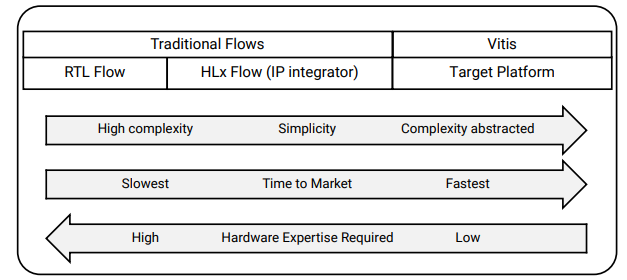
\includegraphics[width=0.8\textwidth]{figures/chapter3/alveo_flow_options.png}
  \caption{Alveo Design Flow Options}
  \label{fig:alveo_flow_options}
\end{figure}

Οπότε με την αξιοποίηση της πλατφόρμας Vitis επιτυγχάνουμε ταχύτερη ανάπτυξη υλικολογισμικού, χωρίς την αναγκαιότητα εξειδικευμένης γνώσης σχεδίασης υλικού.

\section{Τύποι μεταβλητών στο HLS}

Η επιλογή κατάλληλων τύπων μεταβλητών στο High-Level Synthesis (HLS) επηρεάζει άμεσα την απόδοση, τη χρήση πόρων και τη συμπεριφορά του παραγόμενου κυκλώματος.
Το Vitis HLS της Xilinx υποστηρίζει διάφορους τύπους δεδομένων τόσο από τη γλώσσα \texttt{C/C++}, όσο και εξειδικευμένους τύπους για χρήση σε hardware και βελτιστοποίηση.

\subsection{Βασικοί Τύποι Δεδομένων C/C++}
Οι απλοί τύποι δεδομένων της γλώσσας C, όπως \texttt{int}, \texttt{float}, \texttt{char}, \texttt{short}, χρησιμοποιούνται κανονικά στο HLS. Ωστόσο, η χρήση τους μπορεί να οδηγήσει σε υπερβολική χρήση πόρων, ειδικά στην περίπτωση κινητής υποδιαστολής (\texttt{float}). Η χρήση τύπων ακέραιης τιμής είναι προτιμότερη για αποτελεσματική υλοποίηση σε FPGA.

\begin{itemize}
  \item \texttt{int}: 32-bit ακέραιος με υπογραφή.
  \item \texttt{unsigned int}: 32-bit θετικός ακέραιος.
  \item \texttt{float}: 32-bit κινητής υποδιαστολής – αποφεύγεται αν δεν είναι απαραίτητο.
  \item \texttt{bool}: Λογική τιμή – συχνά υλοποιείται ως 1 bit flip-flop.
\end{itemize}

\subsection{Arbitrary Precision Types: \texttt{ap\_int} / \texttt{ap\_uint} / \texttt{ap\_fixed}}
Η Vitis HLS παρέχει τύπους ακριβείας bit μέσω της βιβλιοθήκης \texttt{ap\_fixed.h}. Οι τύποι αυτοί επιτρέπουν τον ακριβή καθορισμό του πλάτους bit:

\begin{itemize}
  \item \texttt{ap\_int<N>}: signed integer με πλάτος \(N\) bits  
  \item \texttt{ap\_uint<N>}: unsigned integer με πλάτος \(N\) bits  
\end{itemize}

Επιτρέπουν προσδιορισμό συγκεκριμένου bit-width οπως 6-bit, 17-bit, 234-bit έως και 1024 bits, προσφέροντας ακριβή έλεγχο κατανάλωσης πόρων.
Αυτό το μέγιστο μήκος μπορεί να παρακαμφθεί ρυθμίζοντας την παράμετρο \textbf{AP\_INT\_MAX\_W μέχρι και 4096 bits}.

Οι καθορισμός συγκεκριμένου μήκους ακρίβειας μεταβλητών (arbitrary precision) προσφέρει δύο βασικά πλεονεκτήματα σε σχέση με τους εγγενείς τύπους της C/C++:
\begin{itemize}
  \item \textbf{Ποιοτικότερη υλοποίηση σε υλικό:} Για παράδειγμα, αν απαιτείται ένας πολλαπλασιαστής 17-bit, οι τύποι αυθαίρετης ακρίβειας επιτρέπουν τον ακριβή ορισμό 17-bit στην πράξη.
  Χωρίς αυτούς τους τύπους, μια τέτοια πράξη πολλαπλασιασμού θα έπρεπε να υλοποιηθεί με χρήση 32-bit ακεραίων τύπων, γεγονός που θα οδηγούσε στην κατανάλωση πολλαπλών μονάδων DSP (Digital Signal Processing) στο FPGA.
  \item \textbf{Ακριβής προσομοίωση και ανάλυση σε επίπεδο C++:} Η χρήση τύπων αυθαίρετης ακρίβειας επιτρέπει την εκτέλεση προσομοιώσεων σε C++ με πιστή αναπαράσταση των πραγματικών bit-widths. Αυτό καθιστά δυνατή την επαλήθευση της λειτουργικότητας και της αριθμητικής ακρίβειας του αλγορίθμου προτού προχωρήσει η σύνθεση (synthesis).
\end{itemize}

Επιπλέον, οι τύποι αυθαίρετης ακρίβειας σε C++ δεν παρουσιάζουν τα μειονεκτήματα που εμφανίζονται σε αντίστοιχες υλοποιήσεις σε C:
\begin{itemize}
  \item Οι αυθαίρετοι τύποι της C++ μπορούν να μεταγλωττιστούν από τυπικούς μεταγλωττιστές C++ και δεν απαιτείται ειδικός compiler.
  \item Δεν επηρεάζονται από προβλήματα τύπου "προαγωγής ακεραίων" (integer promotion), τα οποία είναι συνηθισμένα στην C.
\end{itemize}

\subsection{Σύγκριση Floating-Point και Fixed-Point}
Η χρήση floating-point (π.χ. \texttt{float}, \texttt{double}) δεδομένων αυξάνει σημαντικά την πολυπλοκότητα και την κατανάλωση πόρων.
Η χρήση fixed-point arithmetic στην FPGA μπορεί να μειώσει δραστικά την επιβάρυνση στον FPGA, ειδικά σε real-time εφαρμογές επεξεργασίας σήματος.

Παράδειγμα:
\begin{itemize}
  \item Ένας τύπος floating point μπορεί να απαιτεί περίπου απο 1000 εως και 2000 LUTs (Look-Up Tables) για την υλοποίηση ενός απλού πολλαπλασιαστή και αθροιστή.
  \item Απο την άλλη ένα ειδικό fixed poitn ap\_fixed<16,4> μπορεί να χρειάζεται μόνο ~150 LUTs
\end{itemize}

Πλεονεκτήματα ap\_fixed (Fixed‑Point):
\begin{itemize}
  \item \textbf{Αποδοτικότητα υλικού:} Η fixed‑point υλοποίηση χρησιμοποιεί σημαντικά λιγότερους πόρους στο FPGA (LUTs, DSP blocks) από την floating‑point.
  \item \textbf{Ακριβής και προβλέψιμη συμπεριφορά:} Καθώς το bit‑width είναι καθορισμένο, η ακρίβεια και η συμπεριφορά του υπολογισμού είναι γνωστή εκ των προτέρων χωρίς απροσδόκητες συμπεριφορές.
\end{itemize}

Μειονεκτήματα Fixed‑Point:
\begin{itemize}
  \item \textbf{Περιορισμένο δυναμικό εύρος:} Προαπαιτείται να γνωρίζεις εκ των προτέρων το εύρος των τιμών και να στήσεις ανάλογο scaling. Αυτό αυξάνει την πιθανότητα σφαλμάτων overflow ή loss of precision εάν σχεδιαστούν λανθασμένα οι τιμές
\end{itemize}

\subsection{Παράδειγμα Χρήσης}
\begin{lstlisting}[language=C++, caption={Παράδειγμα χρήσης fixed-point τύπων στο Vitis HLS}]
#include <ap_int.h>
#include <ap_fixed.h>
typedef ap_fixed <16,4,AP_RND_CONV> FPGA_FIXED_POINT;

// Fixed point multiplication function
FPGA_FIXED_POINT multiply(FPGA_FIXED_POINT a, FPGA_FIXED_POINT b) {
  return a * b;
  }
\end{lstlisting}

Αυτός ο αλγόριθμος πολλαπλασιασμού χρησιμοποιεί fixed-point τύπo για να μειώσει τους απαιτούμενους πόρους σε σχέση με την αντίστοιχη υλοποίηση που θα είχε σε floating point.
Με την κατάλληλη επιλογή τύπων δεδομένων, ο σχεδιαστής μπορεί να επιτύχει σημαντικά βελτιωμένη απόδοση και βέλτιστη χρήση των διαθέσιμων πόρων του FPGA.


\section{Vivado}
Το Vivado της Xilinx είναι ένα προηγμένο πακέτο λογισμικού για τον σχεδιασμό ψηφιακής λογικής και την υλοποίηση σε FPGA,
το οποίο χρησιμοποιείται από μηχανικούς και ερευνητές για την ανάπτυξη, προσομοίωση, σύνθεση και υλοποίηση σχεδίων RTL σε FPGA της Xilinx.
Το Vivado προσφέρει προηγμένες λειτουργίες του, όπως η ανάλυση χρονισμού, η βελτιστοποίηση ισχύος και ο Ενσωματωμένος Αναλυτής Λογικής (ILA).

Το Vivado παρουσιάστηκε πρώτη φορά τον Απρίλιο του 2012 και είναι ένα ολοκληρωμένο περιβάλλον σχεδιασμού (IDE) με εργαλεία επιπέδου συστήματος-IC που 
βασίζονται σε ένα κοινό κλιμακωτό μοντέλο δεδομένων και ένα κοινό περιβάλλον εντοπισμού σφαλμάτων.
Το Vivado περιλαμβάνει εργαλεία σχεδιασμού σε επίπεδο ηλεκτρονικού συστήματος (ESL) για τη σύνθεση και την επαλήθευση αλγοριθμικής IP βασισμένης σε C,
τυποποιημένη συσκευασία αλγοριθμικής και RTL IP για επαναχρησιμοποίηση, τυποποιημένη σύνδεση IP και ενσωμάτωση συστημάτων όλων των τύπων δομικών στοιχείων
καθώς και επαλήθευση δομικών στοιχείων και συστημάτων. Έχει και δωρεάν έκδοση την ονομαζόμενη WebPACK Edition του Vivado η οποία παρέχει στους σχεδιαστές
μια περιορισμένη έκδοση του περιβάλλοντος σχεδιασμού.

Ο μεταγλωττιστής Vivado High-Level Synthesis επιτρέπει την άμεση στόχευση προγραμμάτων C, C++ και SystemC σε συσκευές Xilinx χωρίς την ανάγκη χειροκίνητης δημιουργίας RTL.
Το Vivado HLS έχει αξιολογηθεί ευρέως ως μέσο αύξησης της παραγωγικότητας των προγραμματιστών και έχει την δυνατότητα να υποστηρίζει κλάσεις, πρότυπα, συναρτήσεις και υπερφόρτωση τελεστών C++.
Επίσης για πρώτη φορά το Vivado 2014.1 εισήγαγε υποστήριξη για την αυτόματη μετατροπή kernel OpenCL σε IP για συσκευές Xilinx.
Τα kernel σε OpenCL ουσιαστικά είναι προγράμματα που εκτελούνται σε διάφορες πλατφόρμες hardware όπως CPU, GPU και FPGA.

To Vivado προσφέρει πολλά add on οπως:
\begin{itemize}
  \item Vivado Simulator
  \item Vivado IP Integrator
  \item Vivado Tcl Store
\end{itemize}

\subsection{Χαρακτηριστικά και Δυνατότητες}

Το Vivado προσφέρει μια σειρά από χαρακτηριστικά και δυνατότητες που το καθιστούν κορυφαίο εργαλείο για σχεδιασμό FPGA:

\begin{itemize}
  \item \textbf{Ενοποιημένο Περιβάλλον Σχεδίασης (IDE):} Παρέχει γραφικό περιβάλλον για σχεδίαση, σύνθεση, προσομοίωση, ανάλυση χρονισμού και υλοποίηση.
  \item \textbf{IP Integrator:} Ενσωμάτωση προκατασκευασμένων IP blocks, διευκολύνοντας τη δημιουργία σύνθετων συστημάτων με drag-και-drop.
  \item \textbf{Ανάλυση Χρονισμού (Timing Analysis):} Προηγμένα εργαλεία για έλεγχο και βελτιστοποίηση χρονισμού, με αυτόματη ανίχνευση κρίσιμων διαδρομών.
  \item \textbf{Βελτιστοποίηση Ισχύος:} Εργαλεία για ανάλυση και μείωση κατανάλωσης ενέργειας σε επίπεδο σχεδίου.
  \item \textbf{Integrated Logic Analyzer (ILA):} Ενσωματωμένος αναλυτής λογικής για αποσφαλμάτωση σε πραγματικό χρόνο απευθείας στο FPGA.
  \item \textbf{Σύνθεση Υψηλού Επιπέδου (HLS):} Υποστήριξη για μετατροπή C/C++/SystemC σε RTL, επιταχύνοντας την ανάπτυξη και βελτιστοποίηση αλγορίθμων.
  \item \textbf{Διαχείριση Περιορισμών (Constraints Management):} Εύκολη εισαγωγή και επεξεργασία περιορισμών χρονισμού, τοποθέτησης και δρομολόγησης.
  \item \textbf{Εργαλεία Επαλήθευσης και Προσομοίωσης:} Ενσωματωμένος προσομοιωτής, υποστήριξη για ModelSim, Verilator και άλλα εργαλεία τρίτων.
  \item \textbf{Υποστήριξη Πολλαπλών Γλωσσών HDL:} VHDL, Verilog, SystemVerilog, καθώς και C/C++ μέσω HLS.
  \item \textbf{Διαχείριση Έργων και Εκδόσεων:} Εργαλεία για οργάνωση, παρακολούθηση και διαχείριση εκδόσεων σχεδίων.
  \item \textbf{Αυτοματοποιημένη Βελτιστοποίηση Πόρων:} Αυτόματη χαρτογράφηση και βελτιστοποίηση χρήσης LUTs, BRAM, DSP slices κ.ά.
  \item \textbf{Υποστήριξη για Σύγχρονες Αρχιτεκτονικές FPGA:} UltraScale, UltraScale+, Zynq SoC, Versal ACAP.
  \item \textbf{Ενσωμάτωση με SDx και Vitis:} Δυνατότητα συνεργασίας με εργαλεία ανάπτυξης λογισμικού και επιτάχυνσης.
  \item \textbf{Δωρεάν WebPACK Edition:} Περιορισμένη έκδοση για μικρότερα έργα και εκπαιδευτική χρήση.
\end{itemize}

Αυτά τα χαρακτηριστικά καθιστούν το Vivado ιδανικό για επαγγελματική ανάπτυξη, έρευνα και εκπαιδευτική χρήση σε έργα που απαιτούν υψηλή απόδοση, αξιοπιστία και ευελιξία.

Για παραδειγμα μπορούμε να ορίσουμε χρονισμούς και καθυστερήσεις εισόδων/εξόδων στο Vivado,
χρησιμοποιούμε το αρχείο XDC (Xilinx Design Constraints). Ένα τυπικό παράδειγμα για ρολόι 100 MHz και καθυστερήσεις εισόδου/εξόδου είναι:

\begin{lstlisting}[language=tcl, caption={Παράδειγμα XDC Constraints}]
# Define a 100 MHz clock
create_clock -period 10.0 [get_ports clk]

# Set input delay constraints
set_input_delay -clock clk 2.0 [get_ports {input_signal}]

# Set output delay constraints
set_output_delay -clock clk 2.5 [get_ports {output_signal}]
\end{lstlisting}

Αυτές οι εντολές διασφαλίζουν ότι το Vivado θα λάβει υπόψη τους χρονισμούς του ρολογιού και τις καθυστερήσεις σημάτων κατά τη σύνθεση και ανάλυση χρονισμού του σχεδίου.

\subsection{Vivado HLS}

Το Vivado High-Level Synthesis (HLS) αποτελεί ένα εργαλείο που εισήγαγε η Xilinx με στόχο να γεφυρώσει το χάσμα μεταξύ λογισμικού και υλικού,
επιτρέποντας τον σχεδιασμό σε γλώσσες υψηλού επιπέδου όπως C, C++ και SystemC, και την αυτόματη μετατροπή τους σε RTL περιγραφές (VHDL/Verilog).
Με τον τρόπο αυτό, οι μηχανικοί λογισμικού μπορούν να περιγράψουν αλγορίθμους και να τους υλοποιήσουν σε FPGA χωρίς την ανάγκη χειροκίνητης ανάπτυξης RTL.

Τα βασικά πλεονεκτήματα του Vivado HLS περιλαμβάνουν:
\begin{itemize}
  \item \textbf{Επιτάχυνση Ανάπτυξης:} Δραματική μείωση του χρόνου σχεδίασης σε σύγκριση με την παραδοσιακή ανάπτυξη RTL.
  \item \textbf{Αυτοματοποιημένη Βελτιστοποίηση:} Υποστήριξη για βελτιστοποίηση χρονισμού, κατανάλωσης ενέργειας και χρήσης πόρων (LUTs, DSPs, BRAMs).
  \item \textbf{Υποστήριξη C++ χαρακτηριστικών:} Κλάσεις, πρότυπα, συναρτήσεις, υπερφόρτωση τελεστών, καθώς και βιβλιοθήκες αριθμητικής αυθαίρετης ακρίβειας (ap\_int, ap\_fixed).
  \item \textbf{Ενσωμάτωση με Vivado Design Suite:} Αυτόματη δημιουργία IP cores που μπορούν να εισαχθούν μέσω του Vivado IP Integrator.
  \item \textbf{Υποστήριξη OpenCL:} Δυνατότητα μετατροπής kernel γραμμένων σε OpenCL σε IP blocks, ανοίγοντας τον δρόμο για ετερογενείς πλατφόρμες επιτάχυνσης.
\end{itemize}

Ένα παράδειγμα κώδικα σε C++ για Vivado HLS φαίνεται παρακάτω:

\begin{lstlisting}[language=C++, caption={Παράδειγμα απλού αθροιστή σε Vivado HLS}]
#include <ap_int.h>

ap_int<8> add(ap_int<8> a, ap_int<8> b) {
    return a + b;
}
\end{lstlisting}

Κατά την εκτέλεση της σύνθεσης, το Vivado HLS μετατρέπει τη συνάρτηση \texttt{add} σε RTL κώδικα (VHDL/Verilog) και
παράγει αναφορές χρήσης πόρων, χρονισμού και κατανάλωσης ενέργειας. Το παραγόμενο IP core μπορεί στη συνέχεια να χρησιμοποιηθεί στο Vivado IP Integrator ως τμήμα ενός μεγαλύτερου συστήματος.

Το Vivado HLS αποτέλεσε το πρώτο ολοκληρωμένο εργαλείο HLS της Xilinx, ωστόσο μετά το 2019 αντικαταστάθηκε από το \textbf{Vitis HLS},
που ενσωματώνεται στο νέο οικοσύστημα ανάπτυξης Vitis. Το Vivado HLS πλέον θεωρείται legacy εργαλείο, αλλά παραμένει σημαντικό διότι έθεσε τα θεμέλια για την εξάπλωση της χρήσης HLS στον σχεδιασμό FPGA.

\section{Vitis HLS}

Το Vitis HLS είναι ένα εργαλείο σύνθεσης υψηλού επιπέδου που επιτρέπει στους χρήστες να γράφουν κώδικα C/C++ ο οποίος στην συνέχεια
μπορεί να συντεθεί και να ρυθμίστεί σε κυκλώματα FPGA. Το Vitis HLS επιτρέπει στους σχεδιαστές να δημιουργούν γρήγορα πρωτότυπα και να βελτιστοποιούν
τα σχέδια FPGA χρησιμοποιώντας γλώσσες υψηλού επιπέδου και αφηρημένα μοντέλα υλικού, τα οποία μπορούν να μειώσουν σημαντικά τον χρόνο και την προσπάθεια ανάπτυξης.

Το Vitis HLS περιλαμβάνει διάφορα παράθυρα, όπως τα παράθυρα Source, Solution, Reports και Console.
Το παράθυρο Source επιτρέπει στους χρήστες να γράφουν και να επεξεργάζονται κώδικα C/C++, ενώ το παράθυρο Solution παρέχει μια
γραφική διεπαφή για τη διαχείριση της ροής σύνθεσης. Το παράθυρο Reports εμφανίζει τα αποτελέσματα της σύνθεσης, συμπεριλαμβανομένων
των αναφορών χρονισμού και χρήσης πόρων, και το παράθυρο Console εμφανίζει την πρόοδο και την κατάσταση της ροής σύνθεσης.

Οι χρήστες έχουν την δυνατότητα να ρυθμίσουν ειδικές οδηγίες \#PRAGMAS στον κώδικα με οδηγίες για να καθορίσουν τον τρόπο με τον οποίο ο κώδικας C/C++ μπορεί να συντεθεί σε κυκλώματα FPGA
με σκοπό να παρέχει διάφορες επιταχύνσεις στην εκτέλεση. Οι οδηγίες αυτές είναι ειδικά σχόλια που παρέχουν πληροφορίες στο εργαλείο σύνθεσης, όπως παράγοντες ξετυλίγματος βρόχων,
στάδια αγωγού και διαμέριση μνήμης.
Το Vitis HLS παρέχει ένα ευρύ φάσμα οδηγιών που μπορούν να χρησιμοποιηθούν για τη βελτιστοποίηση της απόδοσης και της χρήσης των πόρων του σχεδιασμού FPGA.

Γενικά αποτελεί πλέον ένα απο τα πιο ισχυρά εργαλεία για την ανάπτυξη εφαρμογών low power σε FPGA καθώς επιτρέπει στους χρήστες να γράφουν και να συνθέτουν κώδικα C/C++ σε κυκλώματα.
Το Vitis HLS περιλαμβάνει επίσης εργαλεία για τον εντοπισμό σφαλμάτων, την ανάλυση απόδοσης και τη βελτιστοποίηση κώδικα, τα οποία μπορούν να βοηθήσουν τους χρήστες
να βελτιστοποιήσουν την απόδοση και τη χρήση των πόρων των σχεδίων FPGA τους.

Στο πλαίσιο του Vitis, η «κορυφαία λειτουργία» αναφέρεται στην κύρια λειτουργία σε ένα σχέδιο C/C++ που στοχεύει στην επιτάχυνση υλικού χρησιμοποιώντας το Vitis HLS.
Η κορυφαία λειτουργία είναι το σημείο εκκίνησης του σχεδίου και είναι το σημείο όπου ορίζονται οι είσοδοι και οι έξοδοι του σχεδίου.

Η κορυφαία λειτουργία πρέπει να οριστεί ως C-style kernel με χρήση του `extern "C"` και των κατάλληλων HLS pragmas.

\begin{lstlisting}[language=C++, caption={Ορισμός κορυφαίας λειτουργίας στο Vitis HLS}]
extern "C" {
    void kernelBlackScholes(OPTION_TYPE_BOOL optionType[SIZE], FPGA_FIXED_POINT spotprice[SIZE], FPGA_FIXED_POINT strikeprice[SIZE],  FPGA_FIXED_POINT time[SIZE], FPGA_FIXED_POINT optionPrice[SIZE]){
        #pragma HLS INTERFACE m_axi port=optionType bundle=gmem0
        #pragma HLS INTERFACE m_axi port=spotprice bundle=gmem1
        #pragma HLS INTERFACE m_axi port=strikeprice bundle=gmem2
        #pragma HLS INTERFACE m_axi port=time bundle=gmem3
        #pragma HLS INTERFACE m_axi port=optionPrice bundle=gmem4

        static hls::stream<OPTION_TYPE_BOOL> optionTypeStream("read");
        static hls::stream<FPGA_FIXED_POINT> spotpriceStream("read");
        static hls::stream<FPGA_FIXED_POINT> strikepriceStream("read");
        static hls::stream<FPGA_FIXED_POINT> timeStream("read");
        static hls::stream<FPGA_FIXED_POINT> optionStream("write");

        // Add pragmas to the streams
        #pragma HLS STREAM variable=optionTypeStream depth=2
        #pragma HLS STREAM variable=spotpriceStream depth=2
        #pragma HLS STREAM variable=strikepriceStream depth=2
        #pragma HLS STREAM variable=timeStream depth=2
        #pragma HLS STREAM variable=optionStream depth=2

        #pragma HLS DATAFLOW
        read(optionTypeStream,spotpriceStream,strikepriceStream,timeStream,optionType,spotprice,strikeprice,time);
        compute(optionTypeStream,spotpriceStream,strikepriceStream,timeStream,optionStream);
        write(optionStream, optionPrice);
    }
}
\end{lstlisting}
για να υποδείξει ότι είναι η λειτουργία ανώτατου επιπέδου.

Αυτό το χαρακτηριστικό υποδεικνύει στο Vitis HLS να αντιμετωπίσει τη λειτουργία ως μονάδα ανώτατου επιπέδου του σχεδιασμού, η οποία θα συντεθεί σε μονάδα υλικού FPGA.
Η αρχικη συνάρτηση είναι το σημείο εισόδου του σχεδιασμού Vitis HLS και όλες οι θύρες εισόδου και εξόδου της μονάδας υλικού πρέπει να είναι συνδεδεμένες με την κορυφαία λειτουργία.
Η αρχικη συνάρτηση είναι υπεύθυνη για την αρχικοποίηση των απαιτούμενων τιμών εισόδου και την εκκίνηση της μονάδας υλικού
Μόλις η μονάδα υλικού ολοκληρώσει τον υπολογισμό της, η αρχικη συνάρτηση ανακτά τις τιμές εξόδου και τις επιστρέφει στην εφαρμογή λογισμικού.

\subsection{Οδηγίες \#pragma}
Στην πλατφόρμα λογισμικού AMD Vitis™, ένας πυρήνας που ορίζεται στη γλώσσα C/C++ ή OpenCL™ C πρέπει να μεταγλωττιστεί σε επίπεδο μεταφοράς καταχωρητών (RTL) 
που μπορεί να υλοποιηθεί στην προγραμματιζόμενη λογική μιας συσκευής AMD. 
Ο \textbf{μεταγλωττιστής v++} που θα εξηγηθεί σε επόμενο κεφάλαιο αποτελεί την βασικό εργαλείο compiling και καλεί το εργαλείο Vitis High-Level Synthesis (HLS)
για να συνθέσει τον κώδικα RTL από τον πηγαίο κώδικα του πυρήνα.
Το εργαλείο HLS έχει σχεδιαστεί για να λειτουργεί με το Vitis IDE χωρίς αλληλεπίδραση.
Ωστόσο, το εργαλείο HLS παρέχει επίσης pragmas που μπορούν να χρησιμοποιηθούν για τη βελτιστοποίηση του σχεδιασμού,
τη μείωση της καθυστέρησης, τη βελτίωση της απόδοσης διακίνησης και τη μείωση της χρήσης χώρου και πόρων της συσκευής του τελικού κώδικα RTL.
Αυτά τα pragmas μπορούν να προστεθούν απευθείας στον πηγαίο κώδικα του πυρήνα.
Τα pragmas HLS περιλαμβάνουν τους τύπους βελτιστοποίησης που καθορίζονται στον παρακάτω πίνακα:

\begin{longtable}{|p{4cm}|p{10cm}|}
  \caption{Vitis HLS Pragmas και their descriptions} \label{tab:vitis_hls_pragmas}
  \hline
  \textbf{\# Pragma} & \textbf{Description} \\
  \hline
  \textbf{\#pragma HLS aggregate} & Η οδηγία αυτή χρησιμοποιείται για την ομαδοποίηση όλων των στοιχείων
  μιας δομής (struct) σε ένα ενιαίο ευρύ διάνυσμα ωστε να μπορεί να διαβαστεί και να γραφτεί παράλληλα.\\
  \hline
  \textbf{\#pragma HLS alias} & Το Vitis θεωρεί διαφορετικούς  (pointers) ως ανεξάρτητα κανάλια και γενικά 
  dεν παρέχει καμία ανάλυση εξάρτησης. Ωστόσο, σε περιπτώσεις όπου ο κεντρικός υπολογιστής εκχωρεί ένα μόνο buffer
  για πολλαπλούς δείκτες, αυτή η σχέση μπορεί να επικοινωνηθεί μέσω της pragma ή της οδηγίας ALIAS και η ανάλυση εξάρτησης
  μπορεί να διατηρηθεί. Η pragma ALIAS επιτρέπει την ανάλυση εξάρτησης δεδομένων στο Vitis HLS, καθορίζοντας την απόσταση μεταξύ των δεικτών στο buffer.\\
  \hline
  \textbf{\#pragma HLS disaggregate} & Για την αποδόμηση δομών struct.\\
  \hline
  \textbf{\#pragma HLS expression\_balance} & Η C C++ γράφονται ως μια σειρά οδηγιών η οποία οδηγεί σε μια μεγάλη αλυσίδα RTL.
  Οταν έχουμε μικρή περίοδο λειτουργίας αυτό μπορεί να καθυστερήσει την υλοποίηση. Η οδηγία αυτή χρησιμοποιείται για την εξισορρόπηση
  των εκφράσεων αυτών,δημιουργώντας ένα ισορροπημένο δέντρο από αλυσίδες λειτουργιών. Αυτό μπορεί να μειώσει την καθυστέρηση στον σχεδιασμό, αν και μπορεί να απαιτήσει επιπλέον υλικό.\\
  \hline
  \textbf{\#pragma HLS latency} & Kαθορισμός ελάχιστης και μέγιστης καθυστέρησης μιας λειτουργίας σε κύκλους ρολογιού.\\
  \hline
  \textbf{\#pragma HLS performance} & Kαθορισμός στόχων της υλοποίησης. Μπορεί να τεθεί συνολικά ή και σε επίπεδο συνάρτησης\\
  \hline
  \textbf{\#pragma HLS protocol} & Αυτή η οδηγία καθορίζει μια περιοχή πρωτοκόλλου, στην οποία δεν θα εισαχθούν λειτουργίες ρολογιού από το Vitis,
  εκτός εάν καθοριστούν ρητά στον κώδικα. Το Vitis HLS δεν θα εισάγει τιποτα μεταξύ λειτουργιών στην περιοχή, συμπεριλαμβανομένων αυτών που διαβάζουν
  ή γράφουν στα ορίσματα της συνάρτησης. Η σειρά των αναγνώσεων και εγγραφών θα ακολουθείται αυστηρά στο συντεθειμένο RTL.\\
  \hline
  \textbf{\#pragma HLS reset} & Η οδηγία RESET προσθέτει ή απενεργοποιεί θύρες επαναφοράς (reset ports) για συγκεκριμένες μεταβλητές κατάστασης (global ή static).
  Η θύρα επαναφοράς χρησιμοποιείται για την επαναφορά των καταχωρητών και της μνήμης block RAM, που συνδέονται με τη θύρα, σε μια αρχική τιμή κάθε φορά που εφαρμόζεται το σήμα επαναφοράς.
  Σε παγκόσμιο επίπεδο, η παρουσία και η συμπεριφορά της θύρας επαναφοράς RTL ελέγχεται χρησιμοποιώντας τις ρυθμίσεις διαμόρφωσης \texttt{syn.rtl.reset} (ή \texttt{config\_rtl -reset}).
  Οι ρυθμίσεις διαμόρφωσης επαναφοράς περιλαμβάνουν τη δυνατότητα καθορισμού της πολικότητας της επαναφοράς, τον καθορισμό αν η επαναφορά είναι σύγχρονη ή ασύγχρονη,
  αλλά πιο σημαντικά ελέγχουν, μέσω της επιλογής επαναφοράς, ποιοι καταχωρητές επαναφέρονται όταν εφαρμόζεται το σήμα επαναφοράς.\\
  \hline
  \textbf{\#pragma HLS top} & Επισυνάπτει ένα όνομα σε μια συνάρτηση, το οποίο μπορεί στη συνέχεια να χρησιμοποιηθεί με την εντολή set\_top για τη σύνθεση της
  συνάρτησης και οποιωνδήποτε συναρτήσεων καλούνται από το καθορισμένο ανώτατο επίπεδο. Αυτό χρησιμοποιείται συνήθως για τη σύνθεση συναρτήσεων μελών μιας κλάσης σε C/C++.\\
  \hline
  \textbf{\#pragma HLS stable} & Η οδηγία STABLE ενημερώνει το Vitis HLS για τα εξής: Τα δεδομένα που εφαρμόζονται στη θύρα παραμένουν σταθερά
  κατά τη διάρκεια της κανονικής λειτουργίας, αλλά δεν είναι μια σταθερή τιμή που μπορεί να βελτιστοποιηθεί.
  Η εκπομπή από αυτή τη θύρα δεν απαιτείται να καταχωρηθεί. Η pragma ενημερώνει τον μεταγλωττιστή ότι η είσοδος δεν χρειάζεται να διαβαστεί από την πρώτη διαδικασία ροής δεδομένων
  και ότι η έξοδος δεν χρειάζεται να γραφτεί από την τελευταία διαδικασία ροής δεδομένων σε ένα δίκτυο.\\
  \hline
  \textbf{\#pragma HLS inline} & Η οδηγία inline αφαιρεί μια συνάρτηση ως ξεχωριστή οντότητα στην ιεραρχία και την ενσωμάτωνει στο σημείο κλήσης της.
  Με αυτό τον τρόπο η συνάρτηση διαλύεται στo διευθυνση κλήσης και δεν εμφανίζεται πλέον ως ξεχωριστό επίπεδο ιεραρχίας στο RTL.\\
  \hline
  \textbf{\#pragma HLS interface} & Η οδηγία ή η προδιαγραφή INTERFACE υποστηρίζεται μόνο για χρήση στην συνάρτηση ανώτερου επιπέδου
  και δεν μπορεί να χρησιμοποιηθεί για υποσυναρτήσεις του στοιχείου HLS. Καθορίζει τον τρόπο δημιουργίας των θυρών RTL από τα ορίσματα της συνάρτησης
  κατά τη σύνθεση της διεπαφής, όπως περιγράφεται στην ενότητα Ορισμός διεπαφών.\\
  \hline
  \textbf{\#pragma HLS stream} & Χρησιμοποιεί First IN First OUT (FIFO) αντι για RAM Block για την συνεχόμενη μετάδοση πινάκων σε σειριακή μορφή\\
  \hline
  \textbf{\#pragma HLS dataflow} & Οι συναρτήσεις ή οι βρόχοι στην C που έχουν πρόσβαση σε πίνακες πρέπει να ολοκληρώσουν όλες τις προσβάσεις ανάγνωσης/εγγραφής
  στους πίνακες πριν ολοκληρωθούν. Αυτό εμποδίζει την επόμενη συνάρτηση ή βρόχο που καταναλώνει τα δεδομένα να ξεκινήσει τη λειτουργία.
  Η βελτιστοποίηση DATAFLOW επιτρέπει στις λειτουργίες μιας συνάρτησης ή ενός βρόχου να ξεκινήσουν τη λειτουργία πριν η προηγούμενη συνάρτηση ή βρόχος ολοκληρώσει όλες τις λειτουργίες της.\\
  \hline
  \textbf{\#pragma HLS pipeline} & Μειώνει το διάστημα έναρξης για μια συνάρτηση ή έναν βρόχο, επιτρέποντας την ταυτόχρονη εκτέλεση λειτουργιών.
  Ο προεπιλεγμένος τύπος pipeline ορίζεται από την εντολή config\_compile pipeline\_style, αλλά μπορεί να αντικατασταθεί από την οδηγία ή την προδιαγραφή PIPELINE.
  Μια συνάρτηση ή ένας βρόχος σε pipeline μπορεί να επεξεργάζεται νέες εισόδους κάθε <N> κύκλους ρολογιού, όπου <N> είναι το διαστημα εναρξης νεου βρόχου ή συνάρτησης.
  Ένα διάστημα ίσο με 1 επεξεργάζεται μια νέα είσοδο σε κάθε κύκλο ρολογιού.\\
  \hline
  \textbf{\#pragma HLS occurrence} & Η οδηγία αυτη μπορεί να εφαρμοστεί σε μια κλήση συνάρτησης εντός μιας περιοχής.
  Λειτουργεί με κλήσεις συναρτήσεων σε pipeline εντός ενός μπλοκ συνθηκών, όπως μια δήλωση if ή μια δήλωση switch.
  Η οδηγία καθορίζει πόσο συχνά καλείται η γραμμη ελέγχου εντός της τρέχουσας συνάρτησης. Η αναγνώριση μιας συνάρτησης εντός ενός μπλοκ συνθηκών
  επιτρέπει στις συναρτήσεις και τους βρόχους σε αυτήν την περιοχή να αλληλοσυνδέονται με ένα υψηλότερο διάστημα έναρξης που είναι πιο αργό από τη συνάρτηση ή τον βρόχο που τις περικλείει.\\
  \hline
  \textbf{\#pragma HLS unroll} & Το pragma UNROLL χρησιμοποιείται για να ξετυλίξει βρόχους, δημιουργώντας πολλαπλά αντίγραφα του σώματος του βρόχου στο RTL σχέδιο.
  Αυτό επιτρέπει την παράλληλη εκτέλεση των επαναλήψεων του βρόχου, αυξάνοντας σημαντικά την απόδοση και το throughput του σχεδιασμού.
  Μπορεί να εφαρμοστεί είτε σε όλους τους βρόχους είτε σε συγκεκριμένο βαθμό (μερικό ξετύλιγμα).
  Όταν δεν χρησιμοποιείται το pragma UNROLL, ο βρόχος υλοποιείται ως σειριακή λογική που εκτελείται για κάθε επανάληψη.
  Με το ξετύλιγμα, το εργαλείο HLS δημιουργεί πολλαπλά ανεξάρτητα μονοπάτια λογικής, επιτρέποντας την ταυτόχρονη επεξεργασία δεδομένων. \\
  \hline
  \textbf{\#pragma HLS dependence} & Το Vitis HLS ανιχνεύει εξαρτήσεις εντός βρόχων: οι εξαρτήσεις εντός της ίδιας επανάληψης ενός
  βρόχου είναι εξαρτήσεις ανεξάρτητες από τον βρόχο, ενώ οι εξαρτήσεις μεταξύ διαφορετικών επαναλήψεων ενός βρόχου είναι εξαρτήσεις που μεταφέρονται από τον βρόχο.
  Το pragma DEPENDENCE επιτρέπει την παροχή πρόσθετων πληροφορίων για τον ορισμό, την άρνηση εξαρτήσεων βρόχου και την παράλληλη εκτέλεση βρόχων με μικρότερα διαστήματα.\\
  \hline
  \textbf{\#pragma HLS loop\_flatten} & Επιτρέπει τον αποκερματισμό εμφωλευμένων βρόχων σε μια παράλληλη ιεραρχία εκτέλεσης βρόχων για βελτιωμένη καθυστέρηση.
  Στην υλοποίηση RTL, απαιτείται ένας κύκλος ρολογιού για τη μετάβαση από έναν εξωτερικό βρόχο σε έναν εσωτερικό βρόχο και από έναν εσωτερικό βρόχο σε έναν εξωτερικό βρόχο.
  Η ισοπέδωση των ένθετων βρόχων επιτρέπει την βελτιστοποίησή τους ως ενιαίος βρόχος. Αυτό εξοικονομεί κύκλους ρολογιού, επιτρέποντας ενδεχομένως μεγαλύτερη βελτιστοποίηση της λογικής του σώματος του βρόχου.\\
  \hline
  \textbf{\#pragma HLS loop\_merge} & Συγχωνεύει διαδοχικούς βρόχους σε έναν μόνο βρόχο για να μειώσει τη συνολική καθυστέρηση, να αυξήσει την κοινή χρήση και να βελτιώσει τη λογική βελτιστοποίηση.
  Μειώνει τον αριθμό των κύκλων ρολογιού που απαιτούνται στο RTL για τη μετάβαση μεταξύ των υλοποιήσεων του σώματος του βρόχου. Επιτρέπει την παράλληλη υλοποίηση των βρόχων (εάν είναι δυνατόν).
  Η εντολή αυτή θα επιδιώξει να συγχωνεύσει όλους τους βρόχους εντός του πεδίου εφαρμογής στο οποίο έχει τοποθετηθεί.\\
  \hline
  \textbf{\#pragma HLS loop\_tripcount} & To εργαλείο δέν μπορεί να γνωρίζει εκ των προτερων σε καποια σημεία τον αριθμό των επαναλήψεων οπότε αυτος είναι ενας τρόπος για να ενημερώσεις το πρόγραμμα
  για τις μέγιστες πιθανές επαναλήψεις ωστε να βελτιστοποιήση με αυτή την γνώση το παραγόμενο σχέδιο.\\
  \hline
  \textbf{\#pragma HLS array\_partition} & Διαχωρίζει έναν πίνακα σε μικρότερους πίνακες ή μεμονωμένα στοιχεία, ετσι αυξάνει αποτελεσματικά τον αριθμό των θυρών ανάγνωσης και εγγραφής για την αποθήκευση.
  βεελτιώνοντας ενδεχομένως την απόδοση του σχεδιασμού αλλα ταυτόχρονα απαιτεί περισσότερες μνήμες. \\
  \hline
  \textbf{\#pragma HLS array\_reshape} & Το array reshape αναδιαμορφώνει τον πίνακα με κάθετη αναδιάταξη και συνένωση στοιχείων πινάκων αυξάνοντας το πλάτος των bit.
  Αυτό μειώνει τον αριθμό των μπλοκ RAM που καταναλώνονται, παρέχοντας παράλληλα παράλληλη πρόσβαση στα δεδομένα. Δημιουργεί λοιπόν έναν νέο πίνακα με λιγότερα στοιχεία
  αλλά με μεγαλύτερο πλάτος bit, επιτρέποντας την πρόσβαση σε περισσότερα δεδομένα σε έναν μόνο κύκλο ρολογιού. \\
  \hline
  \textbf{\#pragma HLS aggregate} & Το pragma αυτό χρησιμοποιείται για την ομαδοποίηση όλων των στοιχείων μιας δομής
  σε ένα ενιαίο ευρύ διάνυσμα, ώστε να είναι δυνατή η ταυτόχρονη ανάγνωση και εγγραφή όλων των μελών της δομής.
  Η ευθυγράμμιση bit του νέου ευρέος λέξης που προκύπτει μπορεί να συναχθεί από τη σειρά δήλωσης των στοιχείων της δομής.
  Το πρώτο στοιχείο παίρνει το LSB του διανύσματος και το τελικό στοιχείο της δομής ευθυγραμμίζεται με το MSB του διανύσματος. \\
  \hline
  \textbf{\#pragma HLS allocation} & Καθορίζει τους περιορισμούς για την χρήση πόρων. Η οδηγία λοιπόν μπορεί να περιορίσει τον αριθμό των
  περιπτώσεων RTL και των πόρων υλικού που χρησιμοποιούνται για την υλοποίηση συγκεκριμένων συναρτήσεψν, βρόχων ή λειτουργιών. Η οδηγία καθορίζεται στο σώμα μιας συνάρτησης, ενός βρόχου ή μιας περιοχής κώδικα.\\
  \hline
  \textbf{\#pragma HLS bind\_op} & Το Vitis υλοποιεί τις λειτουργίες στον κώδικα χρησιμοποιώντας συγκεκριμένες υλοποιήσεις.
  H bind op καθορίζει ότι για μια συγκεκριμένη μεταβλητή, μια λειτουργία (mul, add, div) πρέπει να αντιστοιχιστεί σε έναν συγκεκριμένο πόρο συσκευής για υλοποίηση στο RTL.
  Εάν το pragma δεν έχει καθοριστεί, το Vitis καθορίζει αυτόματα τους πόρους που θα χρησιμοποιηθούν για τις λειτουργίες.\\
  \hline
  \textbf{\#pragma HLS bind\_storage} & Αυτή η οδηγία εκχωρεί μια μεταβλητή (πίνακα ή όρισμα συνάρτησης) στον κώδικα σε έναν συγκεκριμένο τύπο μνήμης στο RTL.
  Εάν το pragma δεν έχει καθοριστεί, το εργαλείο Vitis HLS καθορίζει τον τύπο μνήμης που θα εκχωρηθεί. Το εργαλείο επίσης υλοποιεί τη μνήμη χρησιμοποιώντας καθορισμένες υλοποιήσεις στο υλικό. \\
  \hline
  \textbf{\#pragma HLS function\_instantiate} & Τέλος η λειτουργία αυτή είναι μια τεχνική βελτιστοποίησης που έχει τα πλεονεκτήματα της διατήρησης της ιεραρχίας των συναρτήσεων,
  αλλά παρέχει μια επιπλέον ισχυρή επιλογή: την εκτέλεση στοχευμένων τοπικών βελτιστοποιήσεων σε συγκεκριμένες περιπτώσεις μιας συνάρτησης.
  Αυτό μπορεί να απλοποιήσει τη λογική ελέγχου γύρω από την κλήση της συνάρτησης και ενδεχομένως να βελτιώσει την καθυστέρηση και την απόδοση. \\
  \hline
\end{longtable}

Στην συνέχεια έπειτα απο την συντομη αναφορά των διάφορων pragmas θα δούμε μερικά απο τα πιο σημαντικά αναλυτικότερα. Αυτά θα είναι:
\begin{itemize}
  \item pipeline
  \item interface
  \item unroll
  \item flatten
  \item array reshape
  \item partition
\end{itemize}

\subsubsection{Pipeline}
Θα ξεκινήσουμε με την pragma \textbf{pipeline} που είναι και μία απο τις πιό σημαντικές κατά την γνώμη μου. Όπως προαναφέραμε επιγραματικά αυτή η εντολή
μειώνει το διάστημα έναρξης για μια συνάρτηση ή έναν βρόχο, επιτρέποντας την ταυτόχρονη εκτέλεση λειτουργιών. Ουσιαστικά η pipeline επιτρέπει την
διοχέτευση ενός βρόχου για την ταυτόχρονη εκτέλεση των λειτουργιών του βρόχου, όπως φαίνεται στο παρακάτω σχήμα. Στο σχήμα παρουσιάζεται η προεπιλεγμένη
διαδοχική λειτουργία, όπου υπάρχουν τρεις κύκλοι ρολογιού μεταξύ κάθε ανάγνωσης εισόδου και απαιτούνται οκτώ κύκλοι ρολογιού πριν εκτελεστεί η τελευταία εγγραφή εξόδου.
Ενώ το δεύτερο σχήμα δείχνει τις λειτουργίες σε σειρά, όπου υπάρχει ένας κύκλος μεταξύ των αναγνώσεων.

\begin{figure}[h!]
  \centering
  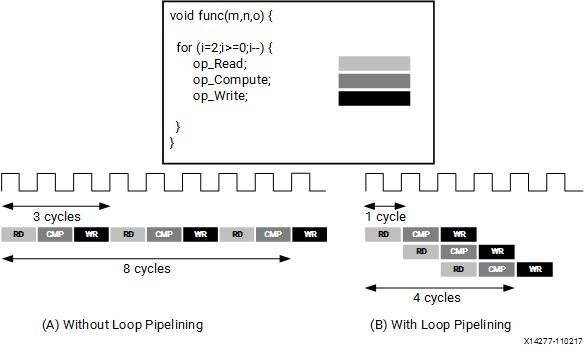
\includegraphics[width=0.8\textwidth]{figures/chapter3/fpga_pipelining.png}
  \caption{FPGA Pragma Pipeline Optimization}
  \label{fig:fpga_pipelining}
\end{figure}

Το παράδειγμα που δίνεται προέρχεται απο τον κώδικα:
\begin{lstlisting}[language=C++, caption={Παράδειγμα χρήσης Pipelining}]
  void example_pipelining(m,n,o){
    #pragma HLS PIPELINE II=1
    for (int i = 2; i >- 0; i--) {
      __operation_read();
      __operation_compute();
      __operation_write();
    }
  }
\end{lstlisting}
  
Ας υποθέσουμε τώρα οτι η κάθε λειτουργία απαιτεί έναν κύκλο ρολογιού για να ολοκληρωθεί Ο(1).
Χωρίς την οδηγία pipeline, ο βρόχος θα απαιτούσε 9 κύκλους ρολογιού (3 για κάθε λειτουργία στον βρόγχο * 3 για τις loop για i=2,1,0) για να ολοκληρωθεί.
Αντίθετα με το pragma pipeline, ο βρόχος μπορεί να ολοκληρωθεί σε 5 κύκλους ρολογιού (3 μεχρι το 3 διάβασμα και 2 για την ολοκλήρωση των υπολοίπων βημάτων του τελευταίου βρόγχου).
Αυτό δηλαδή οδηγεί σε μία σημαντική μείωση του χρόνου εκτέλεσης:

\[
\text{Νο pipeline} = N \times (\text{Κύκλοι Ρολογιού}) = 3 \times 3 = 9 \text{ κύκλοι}
\]
\[
\text{With pipeline} = (\text{Κύκλοι Ρολογιού}) + (\text{Ν-1 Βηματα εκτέλεσης}) = 3 + (3 - 1) = 5 \text{ κύκλοι}
\]
    
Όπως βλέπουμε απο την εξίσωση η χρήση του pipeline δέν θα βοηθήσει μόνο στην περίπτωση που θα είχαμε μόνο 1 κύκλο ρολογιού σε κάθε loop.
Απο εκεί και πέρα το διάστημα της διαφοράς αυξάνεται με ραγδαίους ρυθμούς όσο αυξάνεται ο αριθμός των κύκλων ρολογιού που απαιτούνται για την ολοκλήρωση κάθε βήματος
αλλά και τον αριθμό των επαναλήψεων του βρόχου. Αυτό φαίνεται και στο παρακάτω σχήμα που συγκρίνει την εκτέλεση με και χωρίς pipeline. Με τις χρωματιστές διακεκομένες γραμμές
να απεικονίζουν τις διάφορες επαναλήψεις που χρειάζονται για διαφορετικούς αριθμούς κύκλων ρολογιού μιας συνάρτησης, στον x-αξονα τον αριθμό των επαναλήψεων και στο y να απεικονίζονται
οι συνολικοί κύκλοι εκτέλεξης που απαιτούνται για την ολοκλήρωση.

\begin{figure}[h!]
  \centering
  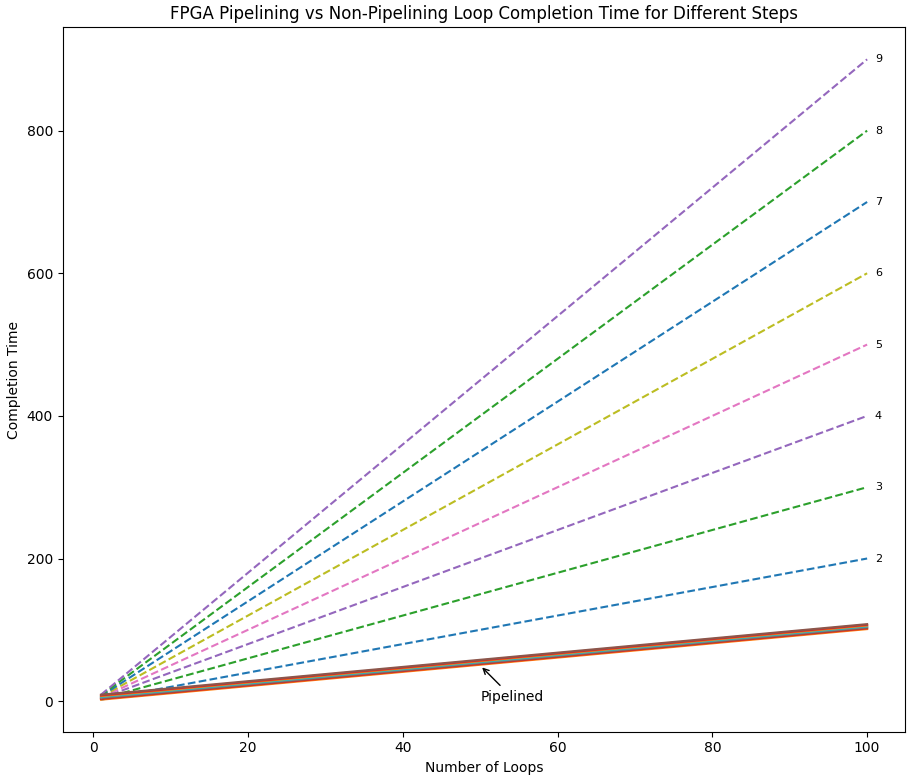
\includegraphics[width=0.7\textwidth]{figures/chapter3/fpga_pipelining_comparison.png}
  \caption{FPGA Pragma Pipeline Conparison}
    \label{fig:fpga_pipelining_comparison}
\end{figure}

Ενδεικτικά δίνονται στο παρακάτω πίνακα οι κύκλου ρολογιού που απαιτούνται για Non Pipelined VS Pipelined αλλά και
το ποσοστό της επιτάχυνσης ανάλογα με τον συνδυασμό των βημάτων και των επαναλήψεων. Όπως βλέπουμε όσο ανεβαίνουν τα βήματα ή οι επαναλήψεις
η επιτάχυνση γίνεται όλο και πιο σημαντική. Σε loop με 100 κύκλους ρολογιού για μια ολοκλήρωση και 20 επαναλήψεις πετυχαίνεται για παράδειγμα
~17 φορές γρηγορότερη εκτέλεση. Φανταστείτε για 1000 ή και παραπάνω επαναλήψεις τι θα μπορούσε να είναι εφικτό! (Θα σας πώ x90!)

\begin{figure}[h!]
  \centering
  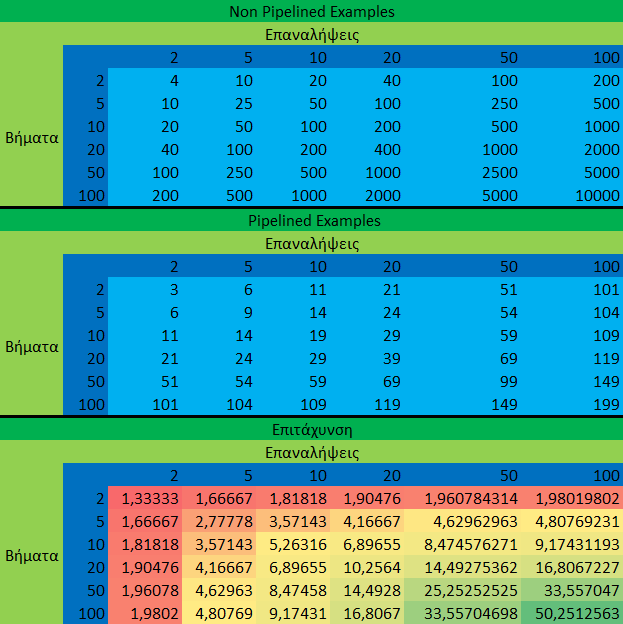
\includegraphics[width=0.7\textwidth]{figures/chapter3/pipelined_speedup.png}
  \caption{Pipeline Speedup}
    \label{fig:pipelined_speedup}
\end{figure}

\subsubsection{Interface}
Το pragma \textbf{interface} είναι επίσης ένα απο τα πιο σημαντικά και χρησιμοποιείται κάθε φορά για τον καθορισμό του τρόπου με τον οποίο τα ορίσματα της αρχικής συνάρτησης
μετατρέπονται σε θύρες RTL κατά τη σύνθεση της διεπαφής. Για αυτό τον λόγο δέν πρεπει να παραληφθεί και πρέπει να παρουσιαστεί παραπάνω λόγω της σημαντικότητας του.
Οι θύρες στην υλοποίηση RTL προέρχονται από τον τύπο δεδομένων και την κατεύθυνση των ορίσματος της συνάρτησης ανώτατου επιπέδου και της επιστροφής της συνάρτησης.
Αυτές οι θύρες καθορίζονται από το config\_interface ή την οδηγία INTERFACE. Η διεπαφή ορίζει επίσης το πρωτόκολλο ελέγχου εκτέλεσης του στοιχείου HLS,
όπως περιγράφεται στα πρωτόκολλα ελέγχου σε επίπεδο μπλοκ. Το πρωτόκολλο ελέγχου καθορίζει πότε το στοιχείο HLS ξεκινά την εκτέλεση και πότε το μπλοκ ολοκληρώνει
τη λειτουργία του, είναι αδρανές και έτοιμο για νέες εισόδους. Η οδηγία είναι η ακόλουθη:

\begin{lstlisting}[language=C++, caption={Οδηγία Interface}]
  #pragma HLS interface mode=<mode> port=<name> direct_io=<value>[OPTIONS]
\end{lstlisting}

Για το όρισμα mode έχουμε αρχικά 3 βασικές διαχωρήσεις πρωτοκόλων και πολλές επιλογές για την κάθε μια οι οποίες είναι οι ακόλουθες επιλογές:
\begin{itemize}
  \item \textbf{Πρωτόκολλα Διεπαφής Port Level:}
      \begin{itemize}
          \item \textbf{ap\_none}: Χωρίς πρωτόκολλο θύρας. Η διεπαφή είναι μια απλή θύρα δεδομένων.
          \item \textbf{ap\_vld}: Υλοποιεί τη θύρα δεδομένων με ένα σήμα valid που υποδεικνύει πότε τα δεδομένα είναι έγκυρα για ανάγνωση ή εγγραφή.
          \item \textbf{ap\_ack}: Υλοποιεί τη θύρα δεδομένων με ένα σήμα acknowledge για επιβεβαίωση ότι τα δεδομένα διαβάστηκαν ή γράφτηκαν.
          \item \textbf{ap\_hs}: Υλοποιεί τη θύρα δεδομένων και μετα τα δύο σήματα valid και acknowledge για αμφίδρομο handshake που υποδεικνύει πότε τα δεδομένα είναι έγκυρα και πότε έγινε επιβεβαίωση ανάγνωσης/εγγραφής.
          \item \textbf{ap\_ovld}: Υλοποιεί τη θύρα εξόδου δεδομένων με σήμα valid για ένδειξη πότε τα δεδομένα είναι έγκυρα για ανάγνωση ή εγγραφή.
          \item \textbf{direct\_io=<true/false>}: Ορίζει αν το pragma INTERFACE εφαρμόζεται απευθείας στο όρισμα της συνάρτησης. Χρήσιμο για SAXI Lite interface.
          Η κλάση hls::direct\_io επιτρέπει τη δυναμική τροποποίηση των scalar ή memory offset παραμέτρων του kernel κατά την εκτέλεση. 
          Χρησιμοποιείται μόνο σε top-level functions και υποστηρίζει όλα τα port-level πρωτόκολλα (ap\_none, ap\_ack, ap\_vld, ap\_hs). 
          Τα direct\_io streams υλοποιούνται ως wires (όχι FIFO) και υποστηρίζουν blocking/non-blocking read/write, με σύνταξη παρόμοια με HLS streams.
          \item \textbf{ap\_memory}: Υλοποιεί τα ορίσματα πίνακα ως τυπική διεπαφή RAM. Στο Vivado IP integrator η διεπαφή αποτελείται από ξεχωριστές θύρες.
          \item \textbf{bram}: Υλοποιεί τα ορίσματα πίνακα ως τυπική διεπαφή RAM με μία θύρα μνήμης.
          \item \textbf{ap\_fifo}: Υλοποιεί τη θύρα ως μια διεπαφή FIFO με θύρες δεδομένων και σήματα active-Low FIFO empty/full. Χρησιμοποιείται μόνο σε read ή write και δεν υποστηρίζει αμφίδρομη επικοινωνία.
      \end{itemize}
  \item \textbf{Πρωτόκολλα Διεπαφής AXI:}
      \begin{itemize}
          \item \textbf{s\_axilite}: Υλοποιεί τη θύρα ως AXI4-Lite διεπαφή. Το εργαλείο παράγει τα αντίστοιχα αρχεία οδηγούς σε C κατά την εξαγωγή του RTL.
          \item \textbf{m\_axi}: Υλοποιεί τη θύρα ως κλασσική AXI4 διεπαφή. Μπορεί να οριστεί ως 32-bit (βασική προεπιλογή) ή 64-bit μέγεθος θύρας με την εντολή config\_interface -m\_axi\_addr64, ενώ μπορεί να ελεγχθεί και οποιαδήποτε μετατόπιση.
          \item \textbf{axis}: Υλοποιεί τη θύρα ως AXI4 διεπαφή ροής (Stream).
      \end{itemize}
  \item \textbf{Πρωτόκολλα Διεπαφής Block Level Control:}
      \begin{itemize}
          \item \textbf{ap\_ctrl\_chain}: Υλοποιεί σύνολο block-level control ports για έναρξη λειτουργίας, συνέχεια, ένδειξη αδράνειας, ολοκλήρωσης και ετοιμότητας για νέα δεδομένα.
          \item \textbf{ap\_ctrl\_hs}: Υλοποιεί block-level control ports για έναρξη λειτουργίας και ένδειξη idle, done και ετοιμότητας για νέα δεδομένα.
          \item \textbf{ap\_ctrl\_none}: Δεν υλοποιείται block-level I/O πρωτόκολλο.
      \end{itemize}
\end{itemize}

Το όρισμα \textbf{port} καθορίζει το όνομα του ορίσματος της συνάρτησης ή της επιστροφής της συνάρτησης στην οποία εφαρμόζεται η pragma interface.
Το όρισμα \textbf{bundle} καθορίζει το όνομα της ομάδας στην οποία θα ενταχθεί η συγκεκριμένη θύρα. 
Από προεπιλογή, το εργαλείο HLS ομαδοποιεί τα ορίσματα της συνάρτησης σε κοινές θύρες διεπαφής στο RTL.. 
Όλες οι διεπαφές AXI4-Lite (\texttt{s\_axilite}) ομαδοποιούνται σε μία θύρα AXI4-Lite όπου είναι εφικτό, ενώ αντίστοιχα όλες οι διεπαφές AXI4 (\texttt{m\_axi}) ομαδοποιούνται σε μία θύρα AXI4. 
Το όνομα της θύρας προκύπτει αυτόματα από τον συνδυασμό του mode και του bundle ή ορίζεται όπως καθορίζεται με την επιλογή \texttt{-name}.
Στην υλοποίηση μας θα δούμε οτι ο ότι κάθε πίνακας δεδομένων (optionType, spotprice, strikeprice, time, optionPrice) συνδέεται με ξεχωριστή AXI memory interface στο FPGA.
Αυτό επιτρέπει την ταυτόχρονη (παράλληλη) πρόσβαση σε πολλαπλά κανάλια μνήμης, αυξάνοντας το συνολικό throughput της εφαρμογής, καθώς οι μεταφορές δεδομένων δεν μοιράζονται 
την ίδια θύρα και δεν δημιουργούν bottlenecks.

Τα υπόλοιπα ορίσματα όπως το \textbf{channel}, \textbf{clock} και \textbf{depth} αλλά και πολλά αλλα είναι επίσης σημαντικά:

\begin{itemize}
  \item \textbf{channel=<string>}: Ενεργοποιεί πολλαπλά κανάλια σε μια διεπαφή \texttt{m\_axi}, ορίζοντας το channel ID.
  \item \textbf{clock=<name>}: Από προεπιλογή, το ρολόι της διεπαφής AXI4-Lite είναι το ίδιο με το ρολόι του συστήματος.
  Αυτή η επιλογή επιτρέπει τον ορισμό ξεχωριστού ρολογιού για μια διεπαφή AXI4-Lite. Αν χρησιμοποιείται το \texttt{-bundle} για ομαδοποίηση πολλών ορισμάτων σε μία διεπαφή AXI4-Lite,
  το ρολόι χρειάζεται να οριστεί μόνο σε ένα μέλος του bundle.
  \item \textbf{depth=<int>}: Καθορίζει το μέγιστο αριθμό δειγμάτων που θα επεξεργαστεί το test bench.
  Αυτή η ρύθμιση υποδεικνύει το μέγιστο μέγεθος του FIFO που απαιτείται στον verification adapter που δημιουργεί το HLS εργαλείο για την προσομοίωση RTL.
  Η επιλογή αυτή δέχεται απλές εκφράσεις βασισμένες στα ορίσματα της συνάρτησης ανώτατου επιπέδου, π.χ. \texttt{depth=SIZE}.
  \item \textbf{interrupt=<int>}: Χρησιμοποιείται μόνο με ap\_vld/ap\_hs. Ενεργοποιεί τη διαχείριση I/O μέσω interrupt, δημιουργώντας τα αντίστοιχα bits στα ISR και IER στο s\_axilite register file.
  \item \textbf{latency=<value>}: Χρησιμοποιείται σε ap\_memory και m\_axi interfaces. Στο ap\_memory, ορίζει το read latency του RAM (προεπιλογή: 1 κύκλος).
  Στο m\_axi, ορίζει την αναμενόμενη καθυστέρηση της διεπαφής AXI4, επιτρέποντας στο σχέδιο να ξεκινήσει αίτημα στο bus πριν την ανάγνωση/εγγραφή.
  \item \textbf{max\_read\_burst\_length=<int>}: Για m\_axi, ορίζει το μέγιστο αριθμό δεδομένων που διαβάζονται σε burst transfer.
  \item \textbf{max\_write\_burst\_length=<int>}: Για m\_axi, ορίζει το μέγιστο αριθμό δεδομένων που γράφονται σε burst transfer.
  \item \textbf{max\_widen\_bitwidth=<int>}: Ορίζει το μέγιστο bit width για αυτόματη διεύρυνση της διεπαφής, παρακάμπτοντας την global ρύθμιση.
  \item \textbf{name=<string>}: Ορίζει όνομα για το port που θα χρησιμοποιηθεί στο παραγόμενο RTL.
  \item \textbf{num\_read\_outstanding=<int>}: Για m\_axi, ορίζει πόσα read requests μπορούν να γίνουν χωρίς απάντηση πριν το σχέδιο σταματήσει. Απαιτεί εσωτερική FIFO: num\_read\_outstanding*max\_read\_burst\_length*word\_size.
  \item \textbf{num\_write\_outstanding=<int>}: Για m\_axi, ορίζει πόσα write requests μπορούν να γίνουν χωρίς απάντηση πριν το σχέδιο σταματήσει. Απαιτεί εσωτερική FIFO: num\_write\_outstanding*max\_write\_burst\_length*word\_size.
  \item \textbf{offset=<string>}: Ελέγχει το address offset σε s\_axilite και m\_axi interfaces για το συγκεκριμένο port. Στο s\_axilite, <string> είναι η διεύθυνση στο register map. Στο m\_axi, μπορεί να είναι off, direct, slave (default).
  \item \textbf{register}: Προαιρετική λέξη-κλειδί για register των σημάτων και των σχετικών πρωτοκόλλων, ώστε να παραμένουν μέχρι τον τελευταίο κύκλο εκτέλεσης της συνάρτησης. Ισχύει για s\_axilite, ap\_fifo, ap\_none, ap\_hs, ap\_ack, ap\_vld, ap\_ovld.
  \item \textbf{register\_mode=<forward|reverse|both|off>}: Για AXI4-Stream, ορίζει αν τα registers τοποθετούνται στην forward path (TDATA/TVALID), reverse path (TREADY), και στα δύο ή κανένα. Default: both.
  \item \textbf{storage\_impl=<impl>}: Μόνο για s\_axilite. Ορίζει storage implementation (auto, bram, uram). Default: auto.
  \item \textbf{storage\_type=<value>}: Μόνο για ap\_memory. Ορίζει storage type (π.χ. ram\_1p, ram\_2p, ram\_t2p, rom\_1p, rom\_2p, rom\_np).
\end{itemize}

\subsubsection{Unroll}
Μια απο τις πιο σημαντικές οδηγίες είναι και η \texbf{Unroll}. Όπως είπαμε και προηγουμενως δημιουργεί πολλα αντίγραφα επεξεργασίας ενός βρόγχου στο φυσικό σχεδιο
ωστε να επιταχύνει και να επιτρέψει την παράλληλη εκτέλεση των επαναλήψεων. Αυτό αυξάνει σημαντικά την απόδοση και την ταχύτητα ολοκλήρωσης. Υπάρχουν 2 πιθανές 
ένοιες για το unrolling. Πλήρες ή \texbf{μερικό ξετύλιγμα} του βρόχου. Το \texbf{πλήρες ξετύλιγμα} του βρόχου δημιουργεί ένα αντίγραφο του σώματος του βρόχου στο RTL για όλες τις επανάληψεις
του βρόχου, έτσι ώστε \texbf{ολόκληρος ο βρόχος} να μπορεί να εκτελεστεί ταυτόχρονα. 
Τπ μερικό ξετύλιγμα ενός βρόχου επιτρέπει να καθορίστει ένας συντελεστής N, για να δημιουργήσει N αντίγραφα του σώματος του βρόχου και να μειώσει ανάλογα τις επαναλήψεις.
Η μερική εκτύλιξη βρόχου δεν απαιτεί το N να είναι ακέραιος παράγοντας του μέγιστου αριθμού επαναλήψεων του βρόχου.
Το εργαλείο Vitis HLS προσθέτει έναν έλεγχο εξόδου για να διασφαλίσει ότι οι μερικώς εκτυλιγμένοι βρόχοι είναι λειτουργικά πανομοιότυποι με τον αρχικό βρόχο.


Για καλύτερη κατανόηση δίνετε το παράδειγμα του ακόλουθου κώδικα:
\begin{lstlisting}[language=C++, caption={Παράδειγμα χρήσης οδηγίας Unrolling}]
  for(int i = 0; i < X; i++) {
    #pragma HLS unroll factor=2
    a[i] = b[i] + c[i];
  }

  Είναι παρόμοιο με:
  for(int i = 0; i < X; i += 2) {
    a[i] = b[i] + c[i];
    if (i+1 >= X) break;
    a[i+1] = b[i+1] + c[i+1];
  }
\end{lstlisting}

Οταν το Χ δέν είναι γνωστό εκ των προτέρων το σχέδιο προσθέτει έλεγχο σαν το προηγούμενο παράδειγμα ωστε να μήν βγεί το εκτελούμενο πρόγραμμα εκτός ορίων.
Ωστόσο άν οι επαναλήψεις είναι γνωστές και είναι σίγουρο οτι θα είναι \texbf{ακεραιο πολλαπλάσιο του Ν} μπορεί ο προγραμματιστής να ορίσει:
\#pragma HLS unroll factor=<N> skip\_exit\_check off=true δλδ την μεταβλητή \texbf{skip\_exit\_check}.
Αυτό βοηθά στην ελαχιστοποίηση της περιοχής και στην απλοποίηση της λογικής ελέγχου. Οι διαθέσιμες μεταβλητές τις οδηγίας αυτής είναι:

\begin{itemize}
  \item \textbf{factor = <N>}: Ρυθμίση για τον Ν ακέραιο αριθμό ο οποίος είναι διαφορετικός από το μηδέν, υποδεικνύοντας ότι απαιτείται μερική εκτύλιξη.
  Το σώμα του βρόχου επαναλαμβάνεται τον καθορισμένο αριθμό φορών και οι πληροφορίες επανάληψης προσαρμόζονται αναλόγως. \texbf{Εάν δεν καθοριστεί ο παράγοντας factor=, ο βρόχος εκτυλίγεται πλήρως}.
  \item \textbf{skip\_exit\_check}: Η μεταβλητή λέξη-κλειδί αυτή είναι προαιρετική και είναι σε ισχύ μόνο αν οριστεί μερική εκτύλιξη με factor=.
  Η εξάλειψη του ελέγχου εξόδου εξαρτάται από το αν ο αριθμός επαναλήψεων του βρόχου είναι γνωστός ή άγνωστος.
  \item \textbf{off = boolean}: Δέχεται true ή false και απενεργοποιεί ή όχι την εκτέλεση της οδηγίας unroll.
\end{itemize}

\subsubsection{Flatten}
Μία αρκετά χρήσιμη οδηγία είναι και η \texbf{loop flatten} η οποία οπως προαναφέραμε κατακερματίζει εμφολευμένους βρόγχους σε μια ενιαία ιεραρχία. Μοιάζει ακρετά με την unroll και πολύ προγραμματιστές
τείνουν να την συγχέουν. Η διαφορά είναι οτι το flatten δέν δημιουργεί αντίγραφα του σώματος του βρόχου αλλά απλά μετατρέπει τους ένθετους βρόχους σε έναν ενιαίο βρόχο με πολλά βήματα.
Μόνο οι τέλειοι και ημι-τέλειοι βρόγχοι μπορούν να γίνουν flatten. Τα είδη βρόγχων εν συντομία είναι:
\begin{itemize}
  \item \textbf{Τέλειοι Βρόγχοι}: Μόνο ο πιο εσωτερικός βρόχος περιέχει στο σώμα του βρόχου λογική με εκτελέσιμο κώδικα. Δεν υπάρχει λογική μεταξύ των δηλώσεων των βρόχων. Όλα τα όρια των βρόχων είναι σταθερά και γνωστά εκ των προτέρων.
  \item \textbf{Ημι-τέλειοι Βρόγχοι}: Ημιτελές λέγονται αυτοί που μοιάζουν με τους τελειους, δηλαδή μόνο ο πιο εσωτερικός βρόχος περιέχει λογική, επίσης δεν υπάρχει λογική μεταξύ των δηλώσεων των βρόχων, αλλά όμως το εξωτερικό όριο του βρόχου μπορεί να είναι μεταβλητή.
  \item \textbf{Ατελείς Βρόγχοι}:  Ατελείς λεγονται όταν ο εσωτερικός βρόχος έχει μεταβλητά όρια ή το σώμα του βρόχου δεν βρίσκεται αποκλειστικά μόνο στον εσωτερικό βρόγχο.
\end{itemize}

\subsubsection{Array Reshape}
Το array reshape κατέχει ιδιαίτερο ενδιαφέρος καθώς μετατρέπει έναν πίνακα σε έναν νέο με λιγότερα στοιχεία αλλά μεγαλύτερο πλάτος bit,
συνενώνοντας στοιχεία ώστε να αυξάνεται η παράλληλη πρόσβαση και να μειώνεται η χρήση μπλοκ RAM.
Έτσι, περισσότερα δεδομένα μπορούν και διαβάζονται σε έναν κύκλο ρολογιού, βελτιώνοντας την απόδοση και την αποδοτικότητα μνήμης. Για παράδειγμα:

\begin{lstlisting}[language=C++, caption={Παράδειγμα Array Reshaping}]
  void foo (...) {
    int array1[N];
    int array2[N];
    int array3[N];
    #pragma HLS ARRAY_RESHAPE variable=array1 type=block factor=2 dim=1
    #pragma HLS ARRAY_RESHAPE variable=array2 type=cyclic factor=2 dim=1
    #pragma HLS ARRAY_RESHAPE variable=array3 type=complete dim=1
    ...
  }
\end{lstlisting}

Στην εικόνα \ref{fig:array_reshape} παρουσιάζεται η λειτουργία του array reshape για τους τρεις διαφορετικούς τύπους που υποστηρίζονται, δηλαδή:
\begin{enumerate}
  \item \textbf{Μπλοκ}
  \item \textbf{Κυκλική}
  \item \textbf{Πλήρης}
\end{enumerate}

\begin{figure}[h!]
  \centering
  \includegraphics[width=0.8\textwidth]{figures/chapter3/array_reshape.png}
  \caption{Reshaping Arrays}
  \label{fig:array_reshape}
\end{figure}

Ας δούμε τώρα συνολικά τις μεταβλητές - διαθέσιμες ρυθμίσεις για την οδηγία Array Reshaping.

\begin{lstlisting}[language=C++, caption={Οδηγία Array Reshaping}]
  #pragma HLS array\_reshape variable=<name> type=<type>  factor=<int>  dim=<int> off=true
\end{lstlisting}

'Οπου:
\begin{itemize}
  \item \textbf{variable=<name>}: Υποχρεωτικό όρισμα που δείχνει το όνομα του πίνακα προς αναπροσαρμογή.
  \item \textbf{type=<type>}: Καθορίζει τον τρόπο αναδιάταξης του πίνακα, με προεπιλογή την complete και οι διαθέσιμες επιλογές είναι:
  \begin{itemize}
    \item \texttt{block}: Συνενώνει διαδοχικά τα στοιχεία του πίνακα σε ευρύτερα bit fields και συνεχίζει σειριακά στην επόμενη γραμμή.
    Το block reshaping δημιουργεί μικρότερους πίνακες από διαδοχικά blocks του αρχικού πίνακα. Αυτό ουσιαστικά χωρίζει τον πίνακα σε <N> ίσα blocks όπου <N> είναι ο
    ακέραιος που ορίζεται από το factor=, και στη συνέχεια συνενώνει τα <N> blocks σε έναν πίνακα με πλάτος λέξης ίσο με word-width*N.
    \item \texttt{cyclic}: Συνενώνει στοιχεία του πίνακα σε registers με κυκλική σειρά ανάθεσης. Δηλαδή θα πάει Index11, Index21, Index31, Index41, Index12, Index22, ...
    Πιο συγκεκριμένα η οδηγία με cyclic reshaping δημιουργεί μικρότερους πίνακες με διαπλοκή των στοιχείων του αρχικού πίνακα.
    Για παράδειγμα, αν οριστεί factor=3, το στοιχείο 0 ανατίθεται στον πρώτο νέο πίνακα, το στοιχείο 1 στον δεύτερο, το στοιχείο 2 στον τρίτο, και το στοιχείο 3 ξανά στον πρώτο νέο πίνακα.
      Το τελικό αποτέλεσμα είναι μια κάθετη συνένωση των νέων πινάκων σε έναν ενιαίο πίνακα με μεγαλύτερο πλάτος λέξης.
      \item \texttt{complete}: Η complete reshaping αποσυνθέτει τον πίνακα σε προσωρινά μεμονωμένα στοιχεία και στη συνέχεια τα επανασυνθέτει σε έναν πίνακα με ευρύτερη λέξη.
      Για μονοδιάστατο πίνακα αυτό ισοδυναμεί με τη δημιουργία ενός πολύ μεγάλου καταχωρητή (αν ο αρχικός πίνακας είχε N στοιχεία των M bits, το αποτέλεσμα είναι ένας καταχωρητής με N*M bits).
      Αυτός είναι ο προεπιλεγμένος τύπος array reshaping.
  \end{itemize}
  \item \textbf{factor=<int>}: Ορίζει τον αριθμό των στοιχείων που θα συνενωθούν σε κάθε word.
  Καθορίζει σε πόσα τμήματα θα διαιρεθεί ο αρχικός πίνακας.
  Για παράδειγμα, factor=2 διαιρεί τον πίνακα στη μέση και διπλασιάζει το πλάτος bit κάθε στοιχείου, ενώ factor=3 τον χωρίζει σε τρία τμήματα με τριπλάσιο bit-width.
  \item \textbf{dim=<int>}: Καθορίζει τη διάσταση του πίνακα στην οποία εφαρμόζεται το reshape.
  Για πολυδιάστατους πίνακες, η τιμή dim ορίζεται ως ενας ακέραιος από 0 έως <N>, όπου <N> είναι ο αριθμός της διαστάσης του πίνακα.
  Αν οριστεί 0, το reshape εφαρμόζεται σε όλες τις διαστάσεις με τις επιλογές type και factor.Αν οριστεί μη μηδενική τιμή, το reshape εφαρμόζεται μόνο στη συγκεκριμένη διάσταση. Για παράδειγμα, dim=1 εφαρμόζει το reshape μόνο στην πρώτη διάσταση του πίνακα.
  \item \textbf{object}: Λέξη κλειδί που χρησιμοποιείται μόνο για container arrays.
  \item \textbf{off}: Αν ειναι αληθής απενεργοποιεί την επίδραση της pragma.
\end{itemize}

Οι λειτουργίες του array reshaping είναι πάρα πολύ χρήσιμες σε εφαρμογές τεχνητής νουμοσύνης αλλά και σε άλλες εφαρμογές όπως υλοποίηση φίλτρων και σε γενικές εφαρμογές επεξεργασίας σήματος ή εικόνας.
  
\subsubsection{Partition}
Τελευταία χρήσιμη οδηγία που εξηγείται πιο αναλυτικά είναι η \textbf{partition}.
Ουσιαστικά, το pragma \textbf{partition} διαχωρίζει έναν πίνακα σε μικρότερους πίνακες ή μεμονωμένα στοιχεία, με αποτέλεσμα το RTL να περιέχει πολλαπλές μικρές μνήμες ή πολλαπλά registers αντί για μία μεγάλη μνήμη.
Αυτό αυξάνει αποτελεσματικά τον αριθμό των θυρών ανάγνωσης και εγγραφής για την αποθήκευση, βελτιώνοντας τον δυνατότητα διεκπαιρέωσης πράξεων και του σχεδιασμού. Ωστόσο, απαιτεί περισσότερες μνήμες ή καταχωρητές.

Η οδηγία είναι η εξής:
\begin{lstlisting}[language=C++, caption={Οδηγία Partitioning}]
  #pragma HLS array_partition variable=<name> type=<type>  factor=<int>  dim=<int> off=true
\end{lstlisting}

'Οπου:
\begin{itemize}
  \item \textbf{variable=<name>}: Υποχρεωτικό όρισμα που δείχνει το όνομα του πίνακα προς κατακερματισμό.
  \item \textbf{type=<type>}: Καθορίζει τον τρόπο κατακερματισμού του πίνακα, με προεπιλογή την complete και οι διαθέσιμες επιλογές είναι:
  \begin{itemize}
    \item \texttt{block}: Κατακερματισμός του πίνακα σε <N> υποδιάστατους πίνακες.
    Ο πίνακας χωρίζεται σε συνεχόμενα τμήματα, όπου κάθε τμήμα αποτελεί έναν ξεχωριστό υπο-πίνακα. Με factor=3, τα στοιχεία κατανέμονται ως εξής:
    Στοιχεία 0 έως (size/3)-1 τοποθετούνται στον πρώτο υπο-πίνακα.
    Στοιχεία (size/3) έως (2×size/3)-1 τοποθετούνται στον δεύτερο υπο-πίνακα.
    Στοιχεία (2×size/3) έως size-1 τοποθετούνται στον τρίτο υπο-πίνακα.
    \item \texttt{cyclic}: Δημιουργεί μικρότερους πίνακες διαμοιράζοντας τα στοιχεία του αρχικού πίνακα με κυκλικό τρόπο.
    Ο πίνακας κατακερματίζεται κυκλικά τοποθετώντας ένα στοιχείο σε κάθε νέο πίνακα πριν επιστρέψει στον πρώτο πίνακα για να επαναλάβει τον κύκλο, μέχρι να κατακερματιστεί πλήρως ο αρχικός πίνακας. Για παράδειγμα, με factor=3:
    Το στοιχείο 0 ανατίθεται στον πρώτο νέο πίνακα. Το στοιχείο 1 ανατίθεται στον δεύτερο νέο πίνακα.
    Το στοιχείο 2 ανατίθεται στον τρίτο νέο πίνακα. Το στοιχείο 3 ανατίθεται ξανά στον πρώτο νέο πίνακα.
    Αυτό το μοτίβο συνεχίζεται για όλα τα στοιχεία του αρχικού πίνακα.
    \item \texttt{complete}: Αποσυνθέτει τον πίνακα σε μεμονωμένα στοιχεία. Για έναν μονοδιάστατο πίνακα, αυτό αντιστοιχεί στη μετατροπή μιας μνήμης σε μεμονωμένους καταχωρητές.
    Κάθε στοιχείο του αρχικού πίνακα αποθηκεύεται σε ξεχωριστό καταχωρητή ή μικρή μνήμη, επιτρέποντας πλήρη παράλληλη πρόσβαση σε όλα τα στοιχεία ταυτόχρονα.
  \end{itemize}
  \item \textbf{factor=<int>}: Ορίζει τον αριθμό των στοιχείων που θα συνενωθούν σε κάθε word.
  Καθορίζει σε πόσα τμήματα θα διαιρεθεί ο αρχικός πίνακας.
  Για παράδειγμα, factor=2 διαιρεί τον πίνακα στη μέση και διπλασιάζει το πλάτος bit κάθε στοιχείου, ενώ factor=3 τον χωρίζει σε τρία τμήματα με τριπλάσιο bit-width.
  \item \textbf{dim=<int>}: Καθορίζει τη διάσταση του πίνακα στην οποία εφαρμόζεται το reshape.
  Για πολυδιάστατους πίνακες, η τιμή dim ορίζεται ως ενας ακέραιος από 0 έως <N>, όπου <N> είναι ο αριθμός της διαστάσης του πίνακα.
  Αν οριστεί 0, το reshape εφαρμόζεται σε όλες τις διαστάσεις με τις επιλογές type και factor.Αν οριστεί μη μηδενική τιμή, το reshape εφαρμόζεται μόνο στη συγκεκριμένη διάσταση. Για παράδειγμα, dim=1 εφαρμόζει το reshape μόνο στην πρώτη διάσταση του πίνακα.
  \item \textbf{object}: Λέξη κλειδί που χρησιμοποιείται μόνο για container arrays.
  \item \textbf{off}: Αν ειναι αληθής απενεργοποιεί την επίδραση της pragma.
\end{itemize}
    
\subsection{Αλλα χρήσιμες δυνατότητες FPGA}
% TODO: ΝΑ μιλήσω για το dual port που έχει και πως μπορεί να διαβάζει και να στέλνει ταυτόχρονα δεδομένα με το switch
\subsection{Προσομοίωση}
\subsection{Σύνθεση}
\begin{figure}[h!]
  \centering
  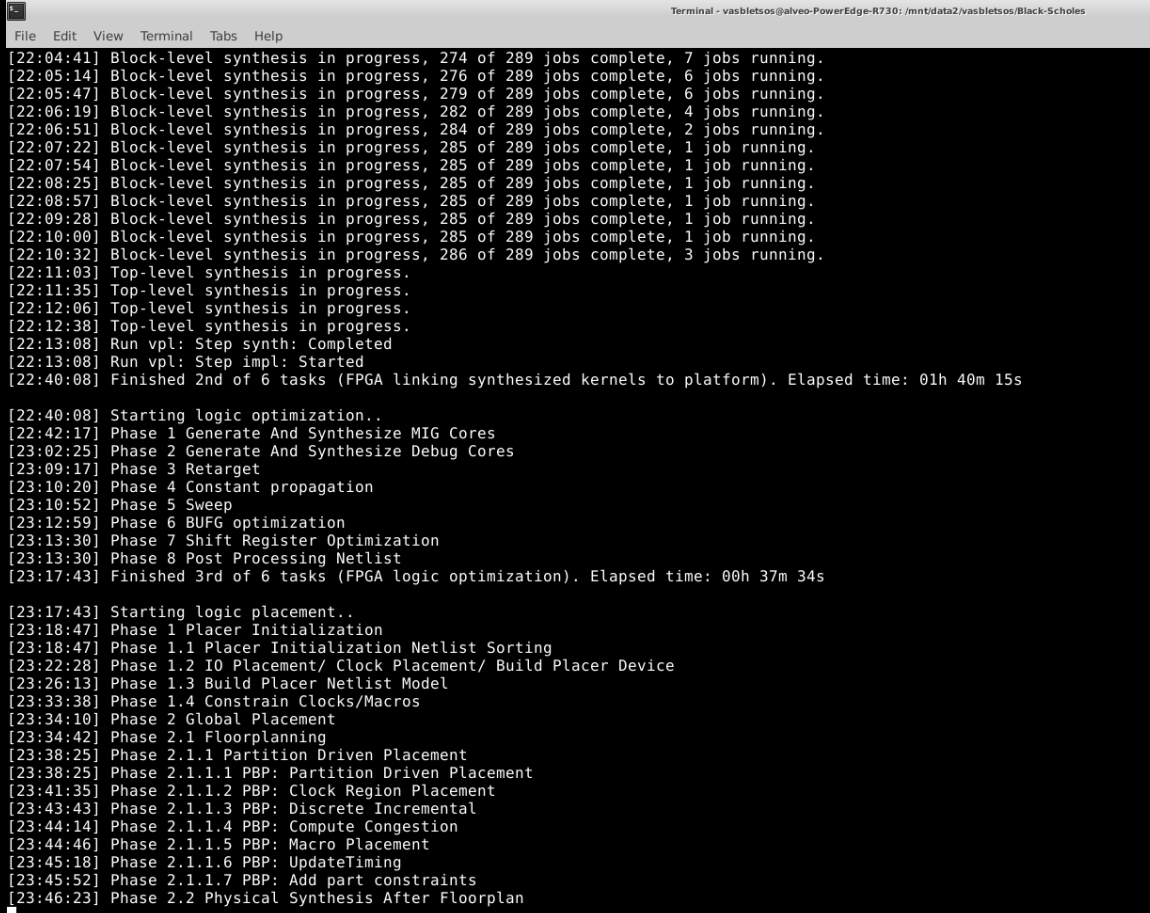
\includegraphics[width=0.8\textwidth]{figures/chapter3/synthesis.png}
  \caption{FPGA Synthesis}
  \label{fig:hw_synthesis_fpga}
\end{figure}

\section{Μεταγλωτιστής V++}